%
% compmod.tex -- Beispiel zum computational mode
%
% (c) 2018 Prof Dr Andreas Müller, Hochschule Rapperswil
%
\documentclass[tikz]{standalone}
\usepackage{times}
\usepackage{txfonts}
\usepackage[utf8]{inputenc} 
\usepackage{graphics}
\usepackage{ifthen}
\usepackage{color}
\usetikzlibrary{arrows,intersections}
\usetikzlibrary{math}
\begin{document} 
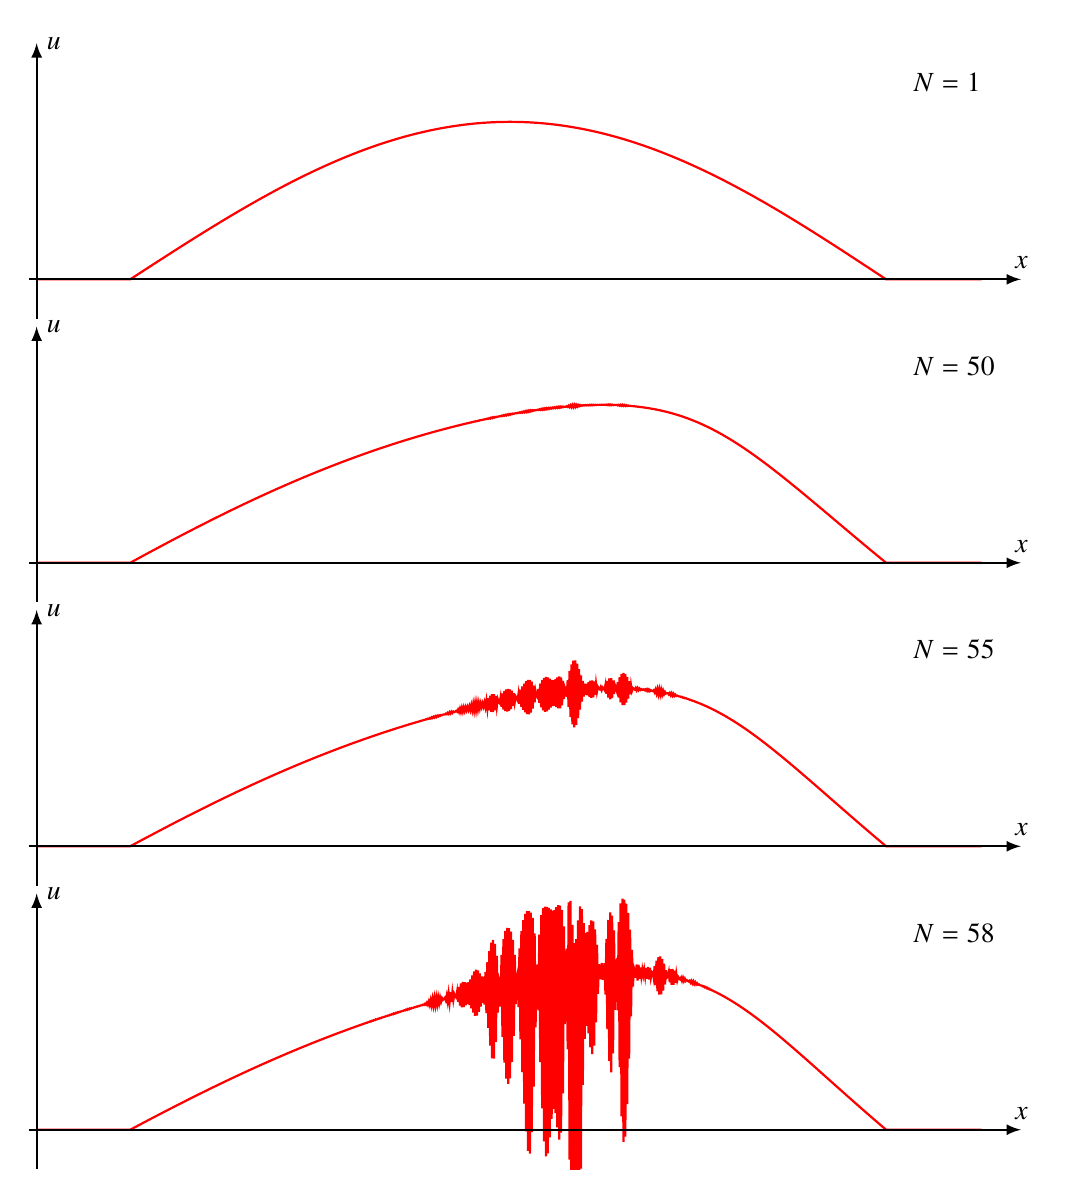
\begin{tikzpicture}[>=latex,thick]

\def\pfada{
\begin{scope}
\clip (0,-0.5) rectangle (12,3);
\draw[color=red] (0,0.0000)
--(0.0120,0.0000)
--(0.0240,0.0000)
--(0.0360,0.0000)
--(0.0480,0.0000)
--(0.0600,0.0000)
--(0.0720,0.0000)
--(0.0840,0.0000)
--(0.0960,0.0000)
--(0.1080,0.0000)
--(0.1200,0.0000)
--(0.1320,0.0000)
--(0.1440,0.0000)
--(0.1560,0.0000)
--(0.1680,0.0000)
--(0.1800,0.0000)
--(0.1920,0.0000)
--(0.2040,0.0000)
--(0.2160,0.0000)
--(0.2280,0.0000)
--(0.2400,0.0000)
--(0.2520,0.0000)
--(0.2640,0.0000)
--(0.2760,0.0000)
--(0.2880,0.0000)
--(0.3000,0.0000)
--(0.3120,0.0000)
--(0.3240,0.0000)
--(0.3360,0.0000)
--(0.3480,0.0000)
--(0.3600,0.0000)
--(0.3720,0.0000)
--(0.3840,0.0000)
--(0.3960,0.0000)
--(0.4080,0.0000)
--(0.4200,0.0000)
--(0.4320,0.0000)
--(0.4440,0.0000)
--(0.4560,0.0000)
--(0.4680,0.0000)
--(0.4800,0.0000)
--(0.4920,0.0000)
--(0.5040,0.0000)
--(0.5160,0.0000)
--(0.5280,0.0000)
--(0.5400,0.0000)
--(0.5520,0.0000)
--(0.5640,0.0000)
--(0.5760,0.0000)
--(0.5880,0.0000)
--(0.6000,0.0000)
--(0.6120,0.0000)
--(0.6240,0.0000)
--(0.6360,0.0000)
--(0.6480,0.0000)
--(0.6600,0.0000)
--(0.6720,0.0000)
--(0.6840,0.0000)
--(0.6960,0.0000)
--(0.7080,0.0000)
--(0.7200,0.0000)
--(0.7320,0.0000)
--(0.7440,0.0000)
--(0.7560,0.0000)
--(0.7680,0.0000)
--(0.7800,0.0000)
--(0.7920,0.0000)
--(0.8040,0.0000)
--(0.8160,0.0000)
--(0.8280,0.0000)
--(0.8400,0.0000)
--(0.8520,0.0000)
--(0.8640,0.0000)
--(0.8760,0.0000)
--(0.8880,0.0000)
--(0.9000,0.0000)
--(0.9120,0.0000)
--(0.9240,0.0000)
--(0.9360,0.0000)
--(0.9480,0.0000)
--(0.9600,0.0000)
--(0.9720,0.0000)
--(0.9840,0.0000)
--(0.9960,0.0000)
--(1.0080,0.0000)
--(1.0200,0.0000)
--(1.0320,0.0000)
--(1.0440,0.0000)
--(1.0560,0.0000)
--(1.0680,0.0000)
--(1.0800,0.0000)
--(1.0920,0.0000)
--(1.1040,0.0000)
--(1.1160,0.0000)
--(1.1280,0.0000)
--(1.1400,0.0000)
--(1.1520,0.0000)
--(1.1640,0.0000)
--(1.1760,0.0000)
--(1.1880,0.0000)
--(1.2000,0.0078)
--(1.2120,0.0156)
--(1.2240,0.0234)
--(1.2360,0.0312)
--(1.2480,0.0390)
--(1.2600,0.0467)
--(1.2720,0.0545)
--(1.2840,0.0623)
--(1.2960,0.0701)
--(1.3080,0.0779)
--(1.3200,0.0857)
--(1.3320,0.0935)
--(1.3440,0.1013)
--(1.3560,0.1090)
--(1.3680,0.1168)
--(1.3800,0.1246)
--(1.3920,0.1324)
--(1.4040,0.1401)
--(1.4160,0.1479)
--(1.4280,0.1557)
--(1.4400,0.1635)
--(1.4520,0.1712)
--(1.4640,0.1790)
--(1.4760,0.1867)
--(1.4880,0.1945)
--(1.5000,0.2023)
--(1.5120,0.2100)
--(1.5240,0.2178)
--(1.5360,0.2255)
--(1.5480,0.2332)
--(1.5600,0.2410)
--(1.5720,0.2487)
--(1.5840,0.2564)
--(1.5960,0.2642)
--(1.6080,0.2719)
--(1.6200,0.2796)
--(1.6320,0.2873)
--(1.6440,0.2950)
--(1.6560,0.3027)
--(1.6680,0.3104)
--(1.6800,0.3181)
--(1.6920,0.3258)
--(1.7040,0.3335)
--(1.7160,0.3412)
--(1.7280,0.3489)
--(1.7400,0.3565)
--(1.7520,0.3642)
--(1.7640,0.3719)
--(1.7760,0.3795)
--(1.7880,0.3872)
--(1.8000,0.3948)
--(1.8120,0.4025)
--(1.8240,0.4101)
--(1.8360,0.4177)
--(1.8480,0.4253)
--(1.8600,0.4329)
--(1.8720,0.4405)
--(1.8840,0.4481)
--(1.8960,0.4557)
--(1.9080,0.4633)
--(1.9200,0.4709)
--(1.9320,0.4785)
--(1.9440,0.4860)
--(1.9560,0.4936)
--(1.9680,0.5011)
--(1.9800,0.5087)
--(1.9920,0.5162)
--(2.0040,0.5237)
--(2.0160,0.5313)
--(2.0280,0.5388)
--(2.0400,0.5463)
--(2.0520,0.5538)
--(2.0640,0.5613)
--(2.0760,0.5687)
--(2.0880,0.5762)
--(2.1000,0.5837)
--(2.1120,0.5911)
--(2.1240,0.5986)
--(2.1360,0.6060)
--(2.1480,0.6134)
--(2.1600,0.6208)
--(2.1720,0.6282)
--(2.1840,0.6356)
--(2.1960,0.6430)
--(2.2080,0.6504)
--(2.2200,0.6578)
--(2.2320,0.6651)
--(2.2440,0.6725)
--(2.2560,0.6798)
--(2.2680,0.6871)
--(2.2800,0.6944)
--(2.2920,0.7018)
--(2.3040,0.7091)
--(2.3160,0.7163)
--(2.3280,0.7236)
--(2.3400,0.7309)
--(2.3520,0.7381)
--(2.3640,0.7454)
--(2.3760,0.7526)
--(2.3880,0.7598)
--(2.4000,0.7670)
--(2.4120,0.7742)
--(2.4240,0.7814)
--(2.4360,0.7886)
--(2.4480,0.7957)
--(2.4600,0.8029)
--(2.4720,0.8100)
--(2.4840,0.8171)
--(2.4960,0.8242)
--(2.5080,0.8313)
--(2.5200,0.8384)
--(2.5320,0.8455)
--(2.5440,0.8526)
--(2.5560,0.8596)
--(2.5680,0.8667)
--(2.5800,0.8737)
--(2.5920,0.8807)
--(2.6040,0.8877)
--(2.6160,0.8947)
--(2.6280,0.9016)
--(2.6400,0.9086)
--(2.6520,0.9155)
--(2.6640,0.9225)
--(2.6760,0.9294)
--(2.6880,0.9363)
--(2.7000,0.9431)
--(2.7120,0.9500)
--(2.7240,0.9569)
--(2.7360,0.9637)
--(2.7480,0.9705)
--(2.7600,0.9774)
--(2.7720,0.9842)
--(2.7840,0.9909)
--(2.7960,0.9977)
--(2.8080,1.0045)
--(2.8200,1.0112)
--(2.8320,1.0179)
--(2.8440,1.0246)
--(2.8560,1.0313)
--(2.8680,1.0380)
--(2.8800,1.0447)
--(2.8920,1.0513)
--(2.9040,1.0579)
--(2.9160,1.0645)
--(2.9280,1.0711)
--(2.9400,1.0777)
--(2.9520,1.0843)
--(2.9640,1.0908)
--(2.9760,1.0974)
--(2.9880,1.1039)
--(3.0000,1.1104)
--(3.0120,1.1169)
--(3.0240,1.1233)
--(3.0360,1.1298)
--(3.0480,1.1362)
--(3.0600,1.1426)
--(3.0720,1.1490)
--(3.0840,1.1554)
--(3.0960,1.1618)
--(3.1080,1.1681)
--(3.1200,1.1744)
--(3.1320,1.1807)
--(3.1440,1.1870)
--(3.1560,1.1933)
--(3.1680,1.1996)
--(3.1800,1.2058)
--(3.1920,1.2120)
--(3.2040,1.2182)
--(3.2160,1.2244)
--(3.2280,1.2306)
--(3.2400,1.2367)
--(3.2520,1.2428)
--(3.2640,1.2489)
--(3.2760,1.2550)
--(3.2880,1.2611)
--(3.3000,1.2671)
--(3.3120,1.2732)
--(3.3240,1.2792)
--(3.3360,1.2852)
--(3.3480,1.2911)
--(3.3600,1.2971)
--(3.3720,1.3030)
--(3.3840,1.3089)
--(3.3960,1.3148)
--(3.4080,1.3207)
--(3.4200,1.3266)
--(3.4320,1.3324)
--(3.4440,1.3382)
--(3.4560,1.3440)
--(3.4680,1.3498)
--(3.4800,1.3555)
--(3.4920,1.3613)
--(3.5040,1.3670)
--(3.5160,1.3727)
--(3.5280,1.3783)
--(3.5400,1.3840)
--(3.5520,1.3896)
--(3.5640,1.3952)
--(3.5760,1.4008)
--(3.5880,1.4064)
--(3.6000,1.4119)
--(3.6120,1.4174)
--(3.6240,1.4229)
--(3.6360,1.4284)
--(3.6480,1.4339)
--(3.6600,1.4393)
--(3.6720,1.4447)
--(3.6840,1.4501)
--(3.6960,1.4555)
--(3.7080,1.4608)
--(3.7200,1.4661)
--(3.7320,1.4714)
--(3.7440,1.4767)
--(3.7560,1.4820)
--(3.7680,1.4872)
--(3.7800,1.4924)
--(3.7920,1.4976)
--(3.8040,1.5028)
--(3.8160,1.5079)
--(3.8280,1.5131)
--(3.8400,1.5182)
--(3.8520,1.5232)
--(3.8640,1.5283)
--(3.8760,1.5333)
--(3.8880,1.5383)
--(3.9000,1.5433)
--(3.9120,1.5483)
--(3.9240,1.5532)
--(3.9360,1.5581)
--(3.9480,1.5630)
--(3.9600,1.5679)
--(3.9720,1.5727)
--(3.9840,1.5775)
--(3.9960,1.5823)
--(4.0080,1.5871)
--(4.0200,1.5918)
--(4.0320,1.5965)
--(4.0440,1.6012)
--(4.0560,1.6059)
--(4.0680,1.6106)
--(4.0800,1.6152)
--(4.0920,1.6198)
--(4.1040,1.6244)
--(4.1160,1.6289)
--(4.1280,1.6334)
--(4.1400,1.6379)
--(4.1520,1.6424)
--(4.1640,1.6469)
--(4.1760,1.6513)
--(4.1880,1.6557)
--(4.2000,1.6601)
--(4.2120,1.6644)
--(4.2240,1.6687)
--(4.2360,1.6730)
--(4.2480,1.6773)
--(4.2600,1.6815)
--(4.2720,1.6858)
--(4.2840,1.6900)
--(4.2960,1.6941)
--(4.3080,1.6983)
--(4.3200,1.7024)
--(4.3320,1.7065)
--(4.3440,1.7106)
--(4.3560,1.7146)
--(4.3680,1.7186)
--(4.3800,1.7226)
--(4.3920,1.7266)
--(4.4040,1.7305)
--(4.4160,1.7344)
--(4.4280,1.7383)
--(4.4400,1.7422)
--(4.4520,1.7460)
--(4.4640,1.7498)
--(4.4760,1.7536)
--(4.4880,1.7573)
--(4.5000,1.7610)
--(4.5120,1.7647)
--(4.5240,1.7684)
--(4.5360,1.7720)
--(4.5480,1.7757)
--(4.5600,1.7792)
--(4.5720,1.7828)
--(4.5840,1.7863)
--(4.5960,1.7898)
--(4.6080,1.7933)
--(4.6200,1.7968)
--(4.6320,1.8002)
--(4.6440,1.8036)
--(4.6560,1.8070)
--(4.6680,1.8103)
--(4.6800,1.8136)
--(4.6920,1.8169)
--(4.7040,1.8202)
--(4.7160,1.8234)
--(4.7280,1.8266)
--(4.7400,1.8298)
--(4.7520,1.8329)
--(4.7640,1.8361)
--(4.7760,1.8391)
--(4.7880,1.8422)
--(4.8000,1.8452)
--(4.8120,1.8482)
--(4.8240,1.8512)
--(4.8360,1.8542)
--(4.8480,1.8571)
--(4.8600,1.8600)
--(4.8720,1.8629)
--(4.8840,1.8657)
--(4.8960,1.8685)
--(4.9080,1.8713)
--(4.9200,1.8740)
--(4.9320,1.8768)
--(4.9440,1.8794)
--(4.9560,1.8821)
--(4.9680,1.8847)
--(4.9800,1.8874)
--(4.9920,1.8899)
--(5.0040,1.8925)
--(5.0160,1.8950)
--(5.0280,1.8975)
--(5.0400,1.9000)
--(5.0520,1.9024)
--(5.0640,1.9048)
--(5.0760,1.9072)
--(5.0880,1.9095)
--(5.1000,1.9118)
--(5.1120,1.9141)
--(5.1240,1.9164)
--(5.1360,1.9186)
--(5.1480,1.9208)
--(5.1600,1.9230)
--(5.1720,1.9251)
--(5.1840,1.9272)
--(5.1960,1.9293)
--(5.2080,1.9314)
--(5.2200,1.9334)
--(5.2320,1.9354)
--(5.2440,1.9373)
--(5.2560,1.9393)
--(5.2680,1.9412)
--(5.2800,1.9430)
--(5.2920,1.9449)
--(5.3040,1.9467)
--(5.3160,1.9485)
--(5.3280,1.9502)
--(5.3400,1.9520)
--(5.3520,1.9537)
--(5.3640,1.9553)
--(5.3760,1.9570)
--(5.3880,1.9586)
--(5.4000,1.9601)
--(5.4120,1.9617)
--(5.4240,1.9632)
--(5.4360,1.9647)
--(5.4480,1.9661)
--(5.4600,1.9676)
--(5.4720,1.9690)
--(5.4840,1.9703)
--(5.4960,1.9716)
--(5.5080,1.9729)
--(5.5200,1.9742)
--(5.5320,1.9755)
--(5.5440,1.9767)
--(5.5560,1.9779)
--(5.5680,1.9790)
--(5.5800,1.9801)
--(5.5920,1.9812)
--(5.6040,1.9823)
--(5.6160,1.9833)
--(5.6280,1.9843)
--(5.6400,1.9853)
--(5.6520,1.9862)
--(5.6640,1.9871)
--(5.6760,1.9880)
--(5.6880,1.9888)
--(5.7000,1.9897)
--(5.7120,1.9904)
--(5.7240,1.9912)
--(5.7360,1.9919)
--(5.7480,1.9926)
--(5.7600,1.9933)
--(5.7720,1.9939)
--(5.7840,1.9945)
--(5.7960,1.9951)
--(5.8080,1.9956)
--(5.8200,1.9961)
--(5.8320,1.9966)
--(5.8440,1.9970)
--(5.8560,1.9975)
--(5.8680,1.9978)
--(5.8800,1.9982)
--(5.8920,1.9985)
--(5.9040,1.9988)
--(5.9160,1.9991)
--(5.9280,1.9993)
--(5.9400,1.9995)
--(5.9520,1.9997)
--(5.9640,1.9998)
--(5.9760,1.9999)
--(5.9880,2.0000)
--(6.0000,2.0000)
--(6.0120,2.0001)
--(6.0240,2.0000)
--(6.0360,2.0000)
--(6.0480,1.9999)
--(6.0600,1.9998)
--(6.0720,1.9997)
--(6.0840,1.9995)
--(6.0960,1.9993)
--(6.1080,1.9991)
--(6.1200,1.9988)
--(6.1320,1.9985)
--(6.1440,1.9982)
--(6.1560,1.9978)
--(6.1680,1.9975)
--(6.1800,1.9970)
--(6.1920,1.9966)
--(6.2040,1.9961)
--(6.2160,1.9956)
--(6.2280,1.9951)
--(6.2400,1.9945)
--(6.2520,1.9939)
--(6.2640,1.9933)
--(6.2760,1.9926)
--(6.2880,1.9919)
--(6.3000,1.9912)
--(6.3120,1.9904)
--(6.3240,1.9896)
--(6.3360,1.9888)
--(6.3480,1.9880)
--(6.3600,1.9871)
--(6.3720,1.9862)
--(6.3840,1.9852)
--(6.3960,1.9843)
--(6.4080,1.9833)
--(6.4200,1.9822)
--(6.4320,1.9812)
--(6.4440,1.9801)
--(6.4560,1.9790)
--(6.4680,1.9778)
--(6.4800,1.9766)
--(6.4920,1.9754)
--(6.5040,1.9742)
--(6.5160,1.9729)
--(6.5280,1.9716)
--(6.5400,1.9702)
--(6.5520,1.9689)
--(6.5640,1.9675)
--(6.5760,1.9660)
--(6.5880,1.9646)
--(6.6000,1.9631)
--(6.6120,1.9616)
--(6.6240,1.9600)
--(6.6360,1.9584)
--(6.6480,1.9568)
--(6.6600,1.9552)
--(6.6720,1.9535)
--(6.6840,1.9518)
--(6.6960,1.9501)
--(6.7080,1.9483)
--(6.7200,1.9465)
--(6.7320,1.9447)
--(6.7440,1.9428)
--(6.7560,1.9409)
--(6.7680,1.9390)
--(6.7800,1.9371)
--(6.7920,1.9351)
--(6.8040,1.9331)
--(6.8160,1.9311)
--(6.8280,1.9290)
--(6.8400,1.9269)
--(6.8520,1.9248)
--(6.8640,1.9226)
--(6.8760,1.9205)
--(6.8880,1.9182)
--(6.9000,1.9160)
--(6.9120,1.9137)
--(6.9240,1.9114)
--(6.9360,1.9091)
--(6.9480,1.9067)
--(6.9600,1.9043)
--(6.9720,1.9019)
--(6.9840,1.8995)
--(6.9960,1.8970)
--(7.0080,1.8945)
--(7.0200,1.8919)
--(7.0320,1.8894)
--(7.0440,1.8868)
--(7.0560,1.8841)
--(7.0680,1.8815)
--(7.0800,1.8788)
--(7.0920,1.8761)
--(7.1040,1.8733)
--(7.1160,1.8706)
--(7.1280,1.8678)
--(7.1400,1.8649)
--(7.1520,1.8621)
--(7.1640,1.8592)
--(7.1760,1.8563)
--(7.1880,1.8533)
--(7.2000,1.8503)
--(7.2120,1.8473)
--(7.2240,1.8443)
--(7.2360,1.8412)
--(7.2480,1.8381)
--(7.2600,1.8350)
--(7.2720,1.8319)
--(7.2840,1.8287)
--(7.2960,1.8255)
--(7.3080,1.8223)
--(7.3200,1.8190)
--(7.3320,1.8157)
--(7.3440,1.8124)
--(7.3560,1.8090)
--(7.3680,1.8057)
--(7.3800,1.8023)
--(7.3920,1.7988)
--(7.4040,1.7954)
--(7.4160,1.7919)
--(7.4280,1.7884)
--(7.4400,1.7848)
--(7.4520,1.7813)
--(7.4640,1.7777)
--(7.4760,1.7740)
--(7.4880,1.7704)
--(7.5000,1.7667)
--(7.5120,1.7630)
--(7.5240,1.7592)
--(7.5360,1.7555)
--(7.5480,1.7517)
--(7.5600,1.7479)
--(7.5720,1.7440)
--(7.5840,1.7401)
--(7.5960,1.7362)
--(7.6080,1.7323)
--(7.6200,1.7284)
--(7.6320,1.7244)
--(7.6440,1.7204)
--(7.6560,1.7163)
--(7.6680,1.7123)
--(7.6800,1.7082)
--(7.6920,1.7041)
--(7.7040,1.6999)
--(7.7160,1.6958)
--(7.7280,1.6916)
--(7.7400,1.6873)
--(7.7520,1.6831)
--(7.7640,1.6788)
--(7.7760,1.6745)
--(7.7880,1.6702)
--(7.8000,1.6658)
--(7.8120,1.6615)
--(7.8240,1.6571)
--(7.8360,1.6526)
--(7.8480,1.6482)
--(7.8600,1.6437)
--(7.8720,1.6392)
--(7.8840,1.6346)
--(7.8960,1.6301)
--(7.9080,1.6255)
--(7.9200,1.6209)
--(7.9320,1.6163)
--(7.9440,1.6116)
--(7.9560,1.6069)
--(7.9680,1.6022)
--(7.9800,1.5975)
--(7.9920,1.5927)
--(8.0040,1.5879)
--(8.0160,1.5831)
--(8.0280,1.5783)
--(8.0400,1.5734)
--(8.0520,1.5685)
--(8.0640,1.5636)
--(8.0760,1.5587)
--(8.0880,1.5537)
--(8.1000,1.5487)
--(8.1120,1.5437)
--(8.1240,1.5387)
--(8.1360,1.5336)
--(8.1480,1.5286)
--(8.1600,1.5235)
--(8.1720,1.5183)
--(8.1840,1.5132)
--(8.1960,1.5080)
--(8.2080,1.5028)
--(8.2200,1.4976)
--(8.2320,1.4923)
--(8.2440,1.4871)
--(8.2560,1.4818)
--(8.2680,1.4765)
--(8.2800,1.4711)
--(8.2920,1.4658)
--(8.3040,1.4604)
--(8.3160,1.4550)
--(8.3280,1.4496)
--(8.3400,1.4441)
--(8.3520,1.4386)
--(8.3640,1.4331)
--(8.3760,1.4276)
--(8.3880,1.4221)
--(8.4000,1.4165)
--(8.4120,1.4109)
--(8.4240,1.4053)
--(8.4360,1.3997)
--(8.4480,1.3940)
--(8.4600,1.3883)
--(8.4720,1.3827)
--(8.4840,1.3769)
--(8.4960,1.3712)
--(8.5080,1.3654)
--(8.5200,1.3596)
--(8.5320,1.3538)
--(8.5440,1.3480)
--(8.5560,1.3422)
--(8.5680,1.3363)
--(8.5800,1.3304)
--(8.5920,1.3245)
--(8.6040,1.3186)
--(8.6160,1.3126)
--(8.6280,1.3067)
--(8.6400,1.3007)
--(8.6520,1.2946)
--(8.6640,1.2886)
--(8.6760,1.2826)
--(8.6880,1.2765)
--(8.7000,1.2704)
--(8.7120,1.2643)
--(8.7240,1.2582)
--(8.7360,1.2520)
--(8.7480,1.2458)
--(8.7600,1.2396)
--(8.7720,1.2334)
--(8.7840,1.2272)
--(8.7960,1.2209)
--(8.8080,1.2147)
--(8.8200,1.2084)
--(8.8320,1.2021)
--(8.8440,1.1957)
--(8.8560,1.1894)
--(8.8680,1.1830)
--(8.8800,1.1767)
--(8.8920,1.1703)
--(8.9040,1.1638)
--(8.9160,1.1574)
--(8.9280,1.1509)
--(8.9400,1.1445)
--(8.9520,1.1380)
--(8.9640,1.1315)
--(8.9760,1.1249)
--(8.9880,1.1184)
--(9.0000,1.1118)
--(9.0120,1.1053)
--(9.0240,1.0987)
--(9.0360,1.0920)
--(9.0480,1.0854)
--(9.0600,1.0788)
--(9.0720,1.0721)
--(9.0840,1.0654)
--(9.0960,1.0587)
--(9.1080,1.0520)
--(9.1200,1.0453)
--(9.1320,1.0385)
--(9.1440,1.0317)
--(9.1560,1.0250)
--(9.1680,1.0182)
--(9.1800,1.0114)
--(9.1920,1.0045)
--(9.2040,0.9977)
--(9.2160,0.9908)
--(9.2280,0.9839)
--(9.2400,0.9770)
--(9.2520,0.9701)
--(9.2640,0.9632)
--(9.2760,0.9563)
--(9.2880,0.9493)
--(9.3000,0.9424)
--(9.3120,0.9354)
--(9.3240,0.9284)
--(9.3360,0.9214)
--(9.3480,0.9143)
--(9.3600,0.9073)
--(9.3720,0.9002)
--(9.3840,0.8932)
--(9.3960,0.8861)
--(9.4080,0.8790)
--(9.4200,0.8719)
--(9.4320,0.8647)
--(9.4440,0.8576)
--(9.4560,0.8505)
--(9.4680,0.8433)
--(9.4800,0.8361)
--(9.4920,0.8289)
--(9.5040,0.8217)
--(9.5160,0.8145)
--(9.5280,0.8073)
--(9.5400,0.8000)
--(9.5520,0.7928)
--(9.5640,0.7855)
--(9.5760,0.7782)
--(9.5880,0.7709)
--(9.6000,0.7636)
--(9.6120,0.7563)
--(9.6240,0.7490)
--(9.6360,0.7416)
--(9.6480,0.7343)
--(9.6600,0.7269)
--(9.6720,0.7195)
--(9.6840,0.7121)
--(9.6960,0.7047)
--(9.7080,0.6973)
--(9.7200,0.6899)
--(9.7320,0.6825)
--(9.7440,0.6750)
--(9.7560,0.6676)
--(9.7680,0.6601)
--(9.7800,0.6526)
--(9.7920,0.6452)
--(9.8040,0.6377)
--(9.8160,0.6302)
--(9.8280,0.6227)
--(9.8400,0.6151)
--(9.8520,0.6076)
--(9.8640,0.6000)
--(9.8760,0.5925)
--(9.8880,0.5849)
--(9.9000,0.5774)
--(9.9120,0.5698)
--(9.9240,0.5622)
--(9.9360,0.5546)
--(9.9480,0.5470)
--(9.9600,0.5394)
--(9.9720,0.5317)
--(9.9840,0.5241)
--(9.9960,0.5165)
--(10.0080,0.5088)
--(10.0200,0.5012)
--(10.0320,0.4935)
--(10.0440,0.4858)
--(10.0560,0.4781)
--(10.0680,0.4705)
--(10.0800,0.4628)
--(10.0920,0.4551)
--(10.1040,0.4473)
--(10.1160,0.4396)
--(10.1280,0.4319)
--(10.1400,0.4242)
--(10.1520,0.4164)
--(10.1640,0.4087)
--(10.1760,0.4009)
--(10.1880,0.3932)
--(10.2000,0.3854)
--(10.2120,0.3777)
--(10.2240,0.3699)
--(10.2360,0.3621)
--(10.2480,0.3543)
--(10.2600,0.3465)
--(10.2720,0.3387)
--(10.2840,0.3309)
--(10.2960,0.3231)
--(10.3080,0.3153)
--(10.3200,0.3075)
--(10.3320,0.2997)
--(10.3440,0.2918)
--(10.3560,0.2840)
--(10.3680,0.2762)
--(10.3800,0.2683)
--(10.3920,0.2605)
--(10.4040,0.2526)
--(10.4160,0.2448)
--(10.4280,0.2369)
--(10.4400,0.2290)
--(10.4520,0.2212)
--(10.4640,0.2133)
--(10.4760,0.2054)
--(10.4880,0.1976)
--(10.5000,0.1897)
--(10.5120,0.1818)
--(10.5240,0.1739)
--(10.5360,0.1660)
--(10.5480,0.1581)
--(10.5600,0.1503)
--(10.5720,0.1424)
--(10.5840,0.1345)
--(10.5960,0.1266)
--(10.6080,0.1187)
--(10.6200,0.1108)
--(10.6320,0.1029)
--(10.6440,0.0950)
--(10.6560,0.0870)
--(10.6680,0.0791)
--(10.6800,0.0712)
--(10.6920,0.0633)
--(10.7040,0.0554)
--(10.7160,0.0475)
--(10.7280,0.0396)
--(10.7400,0.0317)
--(10.7520,0.0237)
--(10.7640,0.0158)
--(10.7760,0.0079)
--(10.7880,0.0000)
--(10.8000,0.0000)
--(10.8120,0.0000)
--(10.8240,0.0000)
--(10.8360,0.0000)
--(10.8480,0.0000)
--(10.8600,0.0000)
--(10.8720,0.0000)
--(10.8840,0.0000)
--(10.8960,0.0000)
--(10.9080,0.0000)
--(10.9200,0.0000)
--(10.9320,0.0000)
--(10.9440,0.0000)
--(10.9560,0.0000)
--(10.9680,0.0000)
--(10.9800,0.0000)
--(10.9920,0.0000)
--(11.0040,0.0000)
--(11.0160,0.0000)
--(11.0280,0.0000)
--(11.0400,0.0000)
--(11.0520,0.0000)
--(11.0640,0.0000)
--(11.0760,0.0000)
--(11.0880,0.0000)
--(11.1000,0.0000)
--(11.1120,0.0000)
--(11.1240,0.0000)
--(11.1360,0.0000)
--(11.1480,0.0000)
--(11.1600,0.0000)
--(11.1720,0.0000)
--(11.1840,0.0000)
--(11.1960,0.0000)
--(11.2080,0.0000)
--(11.2200,0.0000)
--(11.2320,0.0000)
--(11.2440,0.0000)
--(11.2560,0.0000)
--(11.2680,0.0000)
--(11.2800,0.0000)
--(11.2920,0.0000)
--(11.3040,0.0000)
--(11.3160,0.0000)
--(11.3280,0.0000)
--(11.3400,0.0000)
--(11.3520,0.0000)
--(11.3640,0.0000)
--(11.3760,0.0000)
--(11.3880,0.0000)
--(11.4000,0.0000)
--(11.4120,0.0000)
--(11.4240,0.0000)
--(11.4360,0.0000)
--(11.4480,0.0000)
--(11.4600,0.0000)
--(11.4720,0.0000)
--(11.4840,0.0000)
--(11.4960,0.0000)
--(11.5080,0.0000)
--(11.5200,0.0000)
--(11.5320,0.0000)
--(11.5440,0.0000)
--(11.5560,0.0000)
--(11.5680,0.0000)
--(11.5800,0.0000)
--(11.5920,0.0000)
--(11.6040,0.0000)
--(11.6160,0.0000)
--(11.6280,0.0000)
--(11.6400,0.0000)
--(11.6520,0.0000)
--(11.6640,0.0000)
--(11.6760,0.0000)
--(11.6880,0.0000)
--(11.7000,0.0000)
--(11.7120,0.0000)
--(11.7240,0.0000)
--(11.7360,0.0000)
--(11.7480,0.0000)
--(11.7600,0.0000)
--(11.7720,0.0000)
--(11.7840,0.0000)
--(11.7960,0.0000)
--(11.8080,0.0000)
--(11.8200,0.0000)
--(11.8320,0.0000)
--(11.8440,0.0000)
--(11.8560,0.0000)
--(11.8680,0.0000)
--(11.8800,0.0000)
--(11.8920,0.0000)
--(11.9040,0.0000)
--(11.9160,0.0000)
--(11.9280,0.0000)
--(11.9400,0.0000)
--(11.9520,0.0000)
--(11.9640,0.0000)
--(11.9760,0.0000)
--(11.9880,0.0000)
--(12.0000,0.0000)
;
\end{scope}
\node at (11,2.5) [right] {$N=1$};
}
\def\pfadb{
\begin{scope}
\clip (0,-0.5) rectangle (12,3);
\draw[color=red] (0,0.0000)
--(0.0120,0.0000)
--(0.0240,0.0000)
--(0.0360,0.0000)
--(0.0480,0.0000)
--(0.0600,0.0000)
--(0.0720,0.0000)
--(0.0840,0.0000)
--(0.0960,0.0000)
--(0.1080,0.0000)
--(0.1200,0.0000)
--(0.1320,0.0000)
--(0.1440,0.0000)
--(0.1560,0.0000)
--(0.1680,0.0000)
--(0.1800,0.0000)
--(0.1920,0.0000)
--(0.2040,0.0000)
--(0.2160,0.0000)
--(0.2280,0.0000)
--(0.2400,0.0000)
--(0.2520,0.0000)
--(0.2640,0.0000)
--(0.2760,0.0000)
--(0.2880,0.0000)
--(0.3000,0.0000)
--(0.3120,0.0000)
--(0.3240,0.0000)
--(0.3360,0.0000)
--(0.3480,0.0000)
--(0.3600,0.0000)
--(0.3720,0.0000)
--(0.3840,0.0000)
--(0.3960,0.0000)
--(0.4080,0.0000)
--(0.4200,0.0000)
--(0.4320,0.0000)
--(0.4440,0.0000)
--(0.4560,0.0000)
--(0.4680,0.0000)
--(0.4800,0.0000)
--(0.4920,0.0000)
--(0.5040,0.0000)
--(0.5160,0.0000)
--(0.5280,0.0000)
--(0.5400,0.0000)
--(0.5520,0.0000)
--(0.5640,0.0000)
--(0.5760,0.0000)
--(0.5880,0.0000)
--(0.6000,0.0000)
--(0.6120,0.0000)
--(0.6240,0.0000)
--(0.6360,0.0000)
--(0.6480,0.0000)
--(0.6600,0.0000)
--(0.6720,0.0000)
--(0.6840,0.0000)
--(0.6960,0.0000)
--(0.7080,0.0000)
--(0.7200,0.0000)
--(0.7320,0.0000)
--(0.7440,0.0000)
--(0.7560,0.0000)
--(0.7680,0.0000)
--(0.7800,0.0000)
--(0.7920,0.0000)
--(0.8040,0.0000)
--(0.8160,0.0000)
--(0.8280,0.0000)
--(0.8400,0.0000)
--(0.8520,0.0000)
--(0.8640,0.0000)
--(0.8760,0.0000)
--(0.8880,0.0000)
--(0.9000,0.0000)
--(0.9120,0.0000)
--(0.9240,0.0000)
--(0.9360,0.0000)
--(0.9480,0.0000)
--(0.9600,0.0000)
--(0.9720,0.0000)
--(0.9840,0.0000)
--(0.9960,0.0000)
--(1.0080,0.0000)
--(1.0200,0.0000)
--(1.0320,0.0000)
--(1.0440,0.0000)
--(1.0560,0.0000)
--(1.0680,0.0000)
--(1.0800,0.0000)
--(1.0920,0.0000)
--(1.1040,0.0000)
--(1.1160,0.0000)
--(1.1280,0.0000)
--(1.1400,0.0000)
--(1.1520,0.0000)
--(1.1640,0.0000)
--(1.1760,0.0000)
--(1.1880,0.0000)
--(1.2000,0.0066)
--(1.2120,0.0131)
--(1.2240,0.0197)
--(1.2360,0.0262)
--(1.2480,0.0328)
--(1.2600,0.0393)
--(1.2720,0.0458)
--(1.2840,0.0523)
--(1.2960,0.0589)
--(1.3080,0.0654)
--(1.3200,0.0719)
--(1.3320,0.0784)
--(1.3440,0.0849)
--(1.3560,0.0914)
--(1.3680,0.0979)
--(1.3800,0.1044)
--(1.3920,0.1108)
--(1.4040,0.1173)
--(1.4160,0.1238)
--(1.4280,0.1303)
--(1.4400,0.1367)
--(1.4520,0.1432)
--(1.4640,0.1496)
--(1.4760,0.1561)
--(1.4880,0.1625)
--(1.5000,0.1690)
--(1.5120,0.1754)
--(1.5240,0.1818)
--(1.5360,0.1882)
--(1.5480,0.1947)
--(1.5600,0.2011)
--(1.5720,0.2075)
--(1.5840,0.2139)
--(1.5960,0.2203)
--(1.6080,0.2267)
--(1.6200,0.2331)
--(1.6320,0.2394)
--(1.6440,0.2458)
--(1.6560,0.2522)
--(1.6680,0.2585)
--(1.6800,0.2649)
--(1.6920,0.2712)
--(1.7040,0.2776)
--(1.7160,0.2839)
--(1.7280,0.2902)
--(1.7400,0.2966)
--(1.7520,0.3029)
--(1.7640,0.3092)
--(1.7760,0.3155)
--(1.7880,0.3218)
--(1.8000,0.3281)
--(1.8120,0.3344)
--(1.8240,0.3406)
--(1.8360,0.3469)
--(1.8480,0.3532)
--(1.8600,0.3594)
--(1.8720,0.3657)
--(1.8840,0.3719)
--(1.8960,0.3782)
--(1.9080,0.3844)
--(1.9200,0.3906)
--(1.9320,0.3968)
--(1.9440,0.4030)
--(1.9560,0.4092)
--(1.9680,0.4154)
--(1.9800,0.4216)
--(1.9920,0.4278)
--(2.0040,0.4339)
--(2.0160,0.4401)
--(2.0280,0.4462)
--(2.0400,0.4524)
--(2.0520,0.4585)
--(2.0640,0.4647)
--(2.0760,0.4708)
--(2.0880,0.4769)
--(2.1000,0.4830)
--(2.1120,0.4891)
--(2.1240,0.4952)
--(2.1360,0.5013)
--(2.1480,0.5073)
--(2.1600,0.5134)
--(2.1720,0.5195)
--(2.1840,0.5255)
--(2.1960,0.5316)
--(2.2080,0.5376)
--(2.2200,0.5436)
--(2.2320,0.5496)
--(2.2440,0.5556)
--(2.2560,0.5616)
--(2.2680,0.5676)
--(2.2800,0.5736)
--(2.2920,0.5796)
--(2.3040,0.5855)
--(2.3160,0.5915)
--(2.3280,0.5974)
--(2.3400,0.6034)
--(2.3520,0.6093)
--(2.3640,0.6152)
--(2.3760,0.6211)
--(2.3880,0.6270)
--(2.4000,0.6329)
--(2.4120,0.6388)
--(2.4240,0.6447)
--(2.4360,0.6505)
--(2.4480,0.6564)
--(2.4600,0.6622)
--(2.4720,0.6681)
--(2.4840,0.6739)
--(2.4960,0.6797)
--(2.5080,0.6855)
--(2.5200,0.6913)
--(2.5320,0.6971)
--(2.5440,0.7029)
--(2.5560,0.7087)
--(2.5680,0.7144)
--(2.5800,0.7202)
--(2.5920,0.7259)
--(2.6040,0.7317)
--(2.6160,0.7374)
--(2.6280,0.7431)
--(2.6400,0.7488)
--(2.6520,0.7545)
--(2.6640,0.7602)
--(2.6760,0.7658)
--(2.6880,0.7715)
--(2.7000,0.7772)
--(2.7120,0.7828)
--(2.7240,0.7884)
--(2.7360,0.7941)
--(2.7480,0.7997)
--(2.7600,0.8053)
--(2.7720,0.8109)
--(2.7840,0.8164)
--(2.7960,0.8220)
--(2.8080,0.8276)
--(2.8200,0.8331)
--(2.8320,0.8387)
--(2.8440,0.8442)
--(2.8560,0.8497)
--(2.8680,0.8552)
--(2.8800,0.8607)
--(2.8920,0.8662)
--(2.9040,0.8717)
--(2.9160,0.8772)
--(2.9280,0.8826)
--(2.9400,0.8881)
--(2.9520,0.8935)
--(2.9640,0.8989)
--(2.9760,0.9044)
--(2.9880,0.9098)
--(3.0000,0.9152)
--(3.0120,0.9205)
--(3.0240,0.9259)
--(3.0360,0.9313)
--(3.0480,0.9366)
--(3.0600,0.9420)
--(3.0720,0.9473)
--(3.0840,0.9526)
--(3.0960,0.9579)
--(3.1080,0.9632)
--(3.1200,0.9685)
--(3.1320,0.9738)
--(3.1440,0.9790)
--(3.1560,0.9843)
--(3.1680,0.9895)
--(3.1800,0.9948)
--(3.1920,1.0000)
--(3.2040,1.0052)
--(3.2160,1.0104)
--(3.2280,1.0156)
--(3.2400,1.0207)
--(3.2520,1.0259)
--(3.2640,1.0311)
--(3.2760,1.0362)
--(3.2880,1.0413)
--(3.3000,1.0465)
--(3.3120,1.0516)
--(3.3240,1.0567)
--(3.3360,1.0617)
--(3.3480,1.0668)
--(3.3600,1.0719)
--(3.3720,1.0769)
--(3.3840,1.0820)
--(3.3960,1.0870)
--(3.4080,1.0920)
--(3.4200,1.0970)
--(3.4320,1.1020)
--(3.4440,1.1070)
--(3.4560,1.1120)
--(3.4680,1.1169)
--(3.4800,1.1219)
--(3.4920,1.1268)
--(3.5040,1.1317)
--(3.5160,1.1366)
--(3.5280,1.1415)
--(3.5400,1.1464)
--(3.5520,1.1513)
--(3.5640,1.1562)
--(3.5760,1.1610)
--(3.5880,1.1659)
--(3.6000,1.1707)
--(3.6120,1.1755)
--(3.6240,1.1803)
--(3.6360,1.1851)
--(3.6480,1.1899)
--(3.6600,1.1947)
--(3.6720,1.1994)
--(3.6840,1.2042)
--(3.6960,1.2089)
--(3.7080,1.2136)
--(3.7200,1.2184)
--(3.7320,1.2231)
--(3.7440,1.2277)
--(3.7560,1.2324)
--(3.7680,1.2371)
--(3.7800,1.2417)
--(3.7920,1.2464)
--(3.8040,1.2510)
--(3.8160,1.2556)
--(3.8280,1.2602)
--(3.8400,1.2648)
--(3.8520,1.2694)
--(3.8640,1.2740)
--(3.8760,1.2785)
--(3.8880,1.2831)
--(3.9000,1.2876)
--(3.9120,1.2921)
--(3.9240,1.2966)
--(3.9360,1.3011)
--(3.9480,1.3056)
--(3.9600,1.3101)
--(3.9720,1.3146)
--(3.9840,1.3190)
--(3.9960,1.3234)
--(4.0080,1.3279)
--(4.0200,1.3323)
--(4.0320,1.3367)
--(4.0440,1.3411)
--(4.0560,1.3454)
--(4.0680,1.3498)
--(4.0800,1.3541)
--(4.0920,1.3585)
--(4.1040,1.3628)
--(4.1160,1.3671)
--(4.1280,1.3714)
--(4.1400,1.3757)
--(4.1520,1.3800)
--(4.1640,1.3843)
--(4.1760,1.3885)
--(4.1880,1.3928)
--(4.2000,1.3969)
--(4.2120,1.4012)
--(4.2240,1.4054)
--(4.2360,1.4096)
--(4.2480,1.4137)
--(4.2600,1.4180)
--(4.2720,1.4220)
--(4.2840,1.4263)
--(4.2960,1.4303)
--(4.3080,1.4345)
--(4.3200,1.4385)
--(4.3320,1.4427)
--(4.3440,1.4467)
--(4.3560,1.4508)
--(4.3680,1.4548)
--(4.3800,1.4589)
--(4.3920,1.4629)
--(4.4040,1.4669)
--(4.4160,1.4709)
--(4.4280,1.4749)
--(4.4400,1.4789)
--(4.4520,1.4828)
--(4.4640,1.4869)
--(4.4760,1.4907)
--(4.4880,1.4947)
--(4.5000,1.4986)
--(4.5120,1.5026)
--(4.5240,1.5064)
--(4.5360,1.5103)
--(4.5480,1.5141)
--(4.5600,1.5180)
--(4.5720,1.5218)
--(4.5840,1.5257)
--(4.5960,1.5294)
--(4.6080,1.5333)
--(4.6200,1.5371)
--(4.6320,1.5408)
--(4.6440,1.5446)
--(4.6560,1.5483)
--(4.6680,1.5521)
--(4.6800,1.5558)
--(4.6920,1.5596)
--(4.7040,1.5632)
--(4.7160,1.5670)
--(4.7280,1.5705)
--(4.7400,1.5743)
--(4.7520,1.5779)
--(4.7640,1.5815)
--(4.7760,1.5852)
--(4.7880,1.5887)
--(4.8000,1.5924)
--(4.8120,1.5959)
--(4.8240,1.5996)
--(4.8360,1.6031)
--(4.8480,1.6066)
--(4.8600,1.6102)
--(4.8720,1.6137)
--(4.8840,1.6172)
--(4.8960,1.6206)
--(4.9080,1.6242)
--(4.9200,1.6276)
--(4.9320,1.6311)
--(4.9440,1.6344)
--(4.9560,1.6381)
--(4.9680,1.6412)
--(4.9800,1.6450)
--(4.9920,1.6479)
--(5.0040,1.6518)
--(5.0160,1.6545)
--(5.0280,1.6586)
--(5.0400,1.6612)
--(5.0520,1.6653)
--(5.0640,1.6678)
--(5.0760,1.6719)
--(5.0880,1.6745)
--(5.1000,1.6784)
--(5.1120,1.6811)
--(5.1240,1.6848)
--(5.1360,1.6876)
--(5.1480,1.6911)
--(5.1600,1.6942)
--(5.1720,1.6973)
--(5.1840,1.7008)
--(5.1960,1.7035)
--(5.2080,1.7072)
--(5.2200,1.7096)
--(5.2320,1.7136)
--(5.2440,1.7157)
--(5.2560,1.7199)
--(5.2680,1.7220)
--(5.2800,1.7259)
--(5.2920,1.7283)
--(5.3040,1.7317)
--(5.3160,1.7348)
--(5.3280,1.7373)
--(5.3400,1.7412)
--(5.3520,1.7428)
--(5.3640,1.7476)
--(5.3760,1.7485)
--(5.3880,1.7537)
--(5.4000,1.7543)
--(5.4120,1.7595)
--(5.4240,1.7602)
--(5.4360,1.7651)
--(5.4480,1.7662)
--(5.4600,1.7707)
--(5.4720,1.7720)
--(5.4840,1.7764)
--(5.4960,1.7774)
--(5.5080,1.7824)
--(5.5200,1.7826)
--(5.5320,1.7884)
--(5.5440,1.7877)
--(5.5560,1.7942)
--(5.5680,1.7931)
--(5.5800,1.7997)
--(5.5920,1.7987)
--(5.6040,1.8047)
--(5.6160,1.8045)
--(5.6280,1.8096)
--(5.6400,1.8103)
--(5.6520,1.8145)
--(5.6640,1.8157)
--(5.6760,1.8199)
--(5.6880,1.8205)
--(5.7000,1.8257)
--(5.7120,1.8247)
--(5.7240,1.8319)
--(5.7360,1.8286)
--(5.7480,1.8382)
--(5.7600,1.8325)
--(5.7720,1.8440)
--(5.7840,1.8371)
--(5.7960,1.8489)
--(5.8080,1.8426)
--(5.8200,1.8527)
--(5.8320,1.8489)
--(5.8440,1.8556)
--(5.8560,1.8559)
--(5.8680,1.8581)
--(5.8800,1.8628)
--(5.8920,1.8607)
--(5.9040,1.8693)
--(5.9160,1.8638)
--(5.9280,1.8750)
--(5.9400,1.8675)
--(5.9520,1.8801)
--(5.9640,1.8717)
--(5.9760,1.8847)
--(5.9880,1.8763)
--(6.0000,1.8888)
--(6.0120,1.8813)
--(6.0240,1.8923)
--(6.0360,1.8867)
--(6.0480,1.8952)
--(6.0600,1.8925)
--(6.0720,1.8977)
--(6.0840,1.8986)
--(6.0960,1.8999)
--(6.1080,1.9046)
--(6.1200,1.9022)
--(6.1320,1.9103)
--(6.1440,1.9047)
--(6.1560,1.9157)
--(6.1680,1.9074)
--(6.1800,1.9208)
--(6.1920,1.9101)
--(6.2040,1.9257)
--(6.2160,1.9130)
--(6.2280,1.9302)
--(6.2400,1.9163)
--(6.2520,1.9339)
--(6.2640,1.9205)
--(6.2760,1.9366)
--(6.2880,1.9256)
--(6.3000,1.9382)
--(6.3120,1.9316)
--(6.3240,1.9389)
--(6.3360,1.9380)
--(6.3480,1.9394)
--(6.3600,1.9442)
--(6.3720,1.9401)
--(6.3840,1.9499)
--(6.3960,1.9414)
--(6.4080,1.9548)
--(6.4200,1.9433)
--(6.4320,1.9590)
--(6.4440,1.9458)
--(6.4560,1.9623)
--(6.4680,1.9489)
--(6.4800,1.9650)
--(6.4920,1.9525)
--(6.5040,1.9671)
--(6.5160,1.9563)
--(6.5280,1.9691)
--(6.5400,1.9598)
--(6.5520,1.9715)
--(6.5640,1.9626)
--(6.5760,1.9746)
--(6.5880,1.9646)
--(6.6000,1.9780)
--(6.6120,1.9664)
--(6.6240,1.9811)
--(6.6360,1.9686)
--(6.6480,1.9833)
--(6.6600,1.9719)
--(6.6720,1.9842)
--(6.6840,1.9764)
--(6.6960,1.9835)
--(6.7080,1.9822)
--(6.7200,1.9817)
--(6.7320,1.9886)
--(6.7440,1.9794)
--(6.7560,1.9949)
--(6.7680,1.9775)
--(6.7800,2.0003)
--(6.7920,1.9765)
--(6.8040,2.0042)
--(6.8160,1.9772)
--(6.8280,2.0062)
--(6.8400,1.9797)
--(6.8520,2.0063)
--(6.8640,1.9837)
--(6.8760,2.0049)
--(6.8880,1.9886)
--(6.9000,2.0030)
--(6.9120,1.9932)
--(6.9240,2.0017)
--(6.9360,1.9966)
--(6.9480,2.0016)
--(6.9600,1.9985)
--(6.9720,2.0027)
--(6.9840,1.9992)
--(6.9960,2.0045)
--(7.0080,1.9993)
--(7.0200,2.0063)
--(7.0320,1.9996)
--(7.0440,2.0074)
--(7.0560,2.0005)
--(7.0680,2.0077)
--(7.0800,2.0020)
--(7.0920,2.0072)
--(7.1040,2.0039)
--(7.1160,2.0062)
--(7.1280,2.0058)
--(7.1400,2.0054)
--(7.1520,2.0070)
--(7.1640,2.0052)
--(7.1760,2.0071)
--(7.1880,2.0060)
--(7.2000,2.0061)
--(7.2120,2.0075)
--(7.2240,2.0043)
--(7.2360,2.0092)
--(7.2480,2.0024)
--(7.2600,2.0103)
--(7.2720,2.0012)
--(7.2840,2.0102)
--(7.2960,2.0011)
--(7.3080,2.0087)
--(7.3200,2.0021)
--(7.3320,2.0060)
--(7.3440,2.0037)
--(7.3560,2.0026)
--(7.3680,2.0054)
--(7.3800,1.9991)
--(7.3920,2.0067)
--(7.4040,1.9960)
--(7.4160,2.0072)
--(7.4280,1.9936)
--(7.4400,2.0065)
--(7.4520,1.9922)
--(7.4640,2.0045)
--(7.4760,1.9916)
--(7.4880,2.0014)
--(7.5000,1.9915)
--(7.5120,1.9978)
--(7.5240,1.9914)
--(7.5360,1.9942)
--(7.5480,1.9909)
--(7.5600,1.9908)
--(7.5720,1.9896)
--(7.5840,1.9878)
--(7.5960,1.9876)
--(7.6080,1.9852)
--(7.6200,1.9850)
--(7.6320,1.9827)
--(7.6440,1.9820)
--(7.6560,1.9800)
--(7.6680,1.9788)
--(7.6800,1.9771)
--(7.6920,1.9756)
--(7.7040,1.9738)
--(7.7160,1.9724)
--(7.7280,1.9702)
--(7.7400,1.9691)
--(7.7520,1.9665)
--(7.7640,1.9654)
--(7.7760,1.9627)
--(7.7880,1.9613)
--(7.8000,1.9589)
--(7.8120,1.9568)
--(7.8240,1.9550)
--(7.8360,1.9521)
--(7.8480,1.9510)
--(7.8600,1.9471)
--(7.8720,1.9466)
--(7.8840,1.9421)
--(7.8960,1.9419)
--(7.9080,1.9370)
--(7.9200,1.9367)
--(7.9320,1.9319)
--(7.9440,1.9311)
--(7.9560,1.9268)
--(7.9680,1.9251)
--(7.9800,1.9215)
--(7.9920,1.9189)
--(8.0040,1.9160)
--(8.0160,1.9124)
--(8.0280,1.9101)
--(8.0400,1.9059)
--(8.0520,1.9038)
--(8.0640,1.8994)
--(8.0760,1.8971)
--(8.0880,1.8927)
--(8.1000,1.8900)
--(8.1120,1.8859)
--(8.1240,1.8826)
--(8.1360,1.8788)
--(8.1480,1.8750)
--(8.1600,1.8714)
--(8.1720,1.8673)
--(8.1840,1.8636)
--(8.1960,1.8593)
--(8.2080,1.8555)
--(8.2200,1.8512)
--(8.2320,1.8471)
--(8.2440,1.8428)
--(8.2560,1.8385)
--(8.2680,1.8341)
--(8.2800,1.8296)
--(8.2920,1.8252)
--(8.3040,1.8204)
--(8.3160,1.8160)
--(8.3280,1.8111)
--(8.3400,1.8065)
--(8.3520,1.8014)
--(8.3640,1.7966)
--(8.3760,1.7915)
--(8.3880,1.7866)
--(8.4000,1.7814)
--(8.4120,1.7762)
--(8.4240,1.7710)
--(8.4360,1.7656)
--(8.4480,1.7603)
--(8.4600,1.7547)
--(8.4720,1.7493)
--(8.4840,1.7436)
--(8.4960,1.7380)
--(8.5080,1.7322)
--(8.5200,1.7265)
--(8.5320,1.7206)
--(8.5440,1.7147)
--(8.5560,1.7087)
--(8.5680,1.7027)
--(8.5800,1.6965)
--(8.5920,1.6904)
--(8.6040,1.6841)
--(8.6160,1.6778)
--(8.6280,1.6715)
--(8.6400,1.6650)
--(8.6520,1.6585)
--(8.6640,1.6519)
--(8.6760,1.6453)
--(8.6880,1.6386)
--(8.7000,1.6319)
--(8.7120,1.6251)
--(8.7240,1.6182)
--(8.7360,1.6113)
--(8.7480,1.6043)
--(8.7600,1.5972)
--(8.7720,1.5901)
--(8.7840,1.5830)
--(8.7960,1.5757)
--(8.8080,1.5685)
--(8.8200,1.5611)
--(8.8320,1.5537)
--(8.8440,1.5463)
--(8.8560,1.5388)
--(8.8680,1.5312)
--(8.8800,1.5236)
--(8.8920,1.5159)
--(8.9040,1.5082)
--(8.9160,1.5004)
--(8.9280,1.4926)
--(8.9400,1.4847)
--(8.9520,1.4768)
--(8.9640,1.4688)
--(8.9760,1.4608)
--(8.9880,1.4527)
--(9.0000,1.4446)
--(9.0120,1.4364)
--(9.0240,1.4282)
--(9.0360,1.4199)
--(9.0480,1.4116)
--(9.0600,1.4033)
--(9.0720,1.3949)
--(9.0840,1.3864)
--(9.0960,1.3779)
--(9.1080,1.3694)
--(9.1200,1.3608)
--(9.1320,1.3522)
--(9.1440,1.3436)
--(9.1560,1.3349)
--(9.1680,1.3261)
--(9.1800,1.3174)
--(9.1920,1.3085)
--(9.2040,1.2997)
--(9.2160,1.2908)
--(9.2280,1.2819)
--(9.2400,1.2729)
--(9.2520,1.2639)
--(9.2640,1.2549)
--(9.2760,1.2459)
--(9.2880,1.2368)
--(9.3000,1.2277)
--(9.3120,1.2185)
--(9.3240,1.2093)
--(9.3360,1.2001)
--(9.3480,1.1908)
--(9.3600,1.1816)
--(9.3720,1.1723)
--(9.3840,1.1629)
--(9.3960,1.1536)
--(9.4080,1.1442)
--(9.4200,1.1348)
--(9.4320,1.1253)
--(9.4440,1.1159)
--(9.4560,1.1064)
--(9.4680,1.0969)
--(9.4800,1.0873)
--(9.4920,1.0778)
--(9.5040,1.0682)
--(9.5160,1.0586)
--(9.5280,1.0490)
--(9.5400,1.0393)
--(9.5520,1.0296)
--(9.5640,1.0200)
--(9.5760,1.0102)
--(9.5880,1.0005)
--(9.6000,0.9908)
--(9.6120,0.9810)
--(9.6240,0.9712)
--(9.6360,0.9614)
--(9.6480,0.9516)
--(9.6600,0.9418)
--(9.6720,0.9320)
--(9.6840,0.9221)
--(9.6960,0.9122)
--(9.7080,0.9024)
--(9.7200,0.8925)
--(9.7320,0.8825)
--(9.7440,0.8726)
--(9.7560,0.8627)
--(9.7680,0.8527)
--(9.7800,0.8428)
--(9.7920,0.8328)
--(9.8040,0.8228)
--(9.8160,0.8128)
--(9.8280,0.8028)
--(9.8400,0.7928)
--(9.8520,0.7828)
--(9.8640,0.7728)
--(9.8760,0.7627)
--(9.8880,0.7527)
--(9.9000,0.7426)
--(9.9120,0.7326)
--(9.9240,0.7225)
--(9.9360,0.7124)
--(9.9480,0.7024)
--(9.9600,0.6923)
--(9.9720,0.6822)
--(9.9840,0.6721)
--(9.9960,0.6620)
--(10.0080,0.6519)
--(10.0200,0.6418)
--(10.0320,0.6317)
--(10.0440,0.6216)
--(10.0560,0.6115)
--(10.0680,0.6014)
--(10.0800,0.5912)
--(10.0920,0.5811)
--(10.1040,0.5710)
--(10.1160,0.5609)
--(10.1280,0.5507)
--(10.1400,0.5406)
--(10.1520,0.5305)
--(10.1640,0.5204)
--(10.1760,0.5102)
--(10.1880,0.5001)
--(10.2000,0.4900)
--(10.2120,0.4799)
--(10.2240,0.4698)
--(10.2360,0.4596)
--(10.2480,0.4495)
--(10.2600,0.4394)
--(10.2720,0.4293)
--(10.2840,0.4192)
--(10.2960,0.4091)
--(10.3080,0.3990)
--(10.3200,0.3889)
--(10.3320,0.3788)
--(10.3440,0.3687)
--(10.3560,0.3586)
--(10.3680,0.3485)
--(10.3800,0.3384)
--(10.3920,0.3283)
--(10.4040,0.3183)
--(10.4160,0.3082)
--(10.4280,0.2982)
--(10.4400,0.2881)
--(10.4520,0.2780)
--(10.4640,0.2680)
--(10.4760,0.2580)
--(10.4880,0.2479)
--(10.5000,0.2379)
--(10.5120,0.2279)
--(10.5240,0.2179)
--(10.5360,0.2079)
--(10.5480,0.1979)
--(10.5600,0.1879)
--(10.5720,0.1780)
--(10.5840,0.1680)
--(10.5960,0.1580)
--(10.6080,0.1481)
--(10.6200,0.1381)
--(10.6320,0.1282)
--(10.6440,0.1183)
--(10.6560,0.1084)
--(10.6680,0.0985)
--(10.6800,0.0886)
--(10.6920,0.0787)
--(10.7040,0.0688)
--(10.7160,0.0589)
--(10.7280,0.0491)
--(10.7400,0.0392)
--(10.7520,0.0294)
--(10.7640,0.0196)
--(10.7760,0.0098)
--(10.7880,0.0000)
--(10.8000,0.0000)
--(10.8120,0.0000)
--(10.8240,0.0000)
--(10.8360,0.0000)
--(10.8480,0.0000)
--(10.8600,0.0000)
--(10.8720,0.0000)
--(10.8840,0.0000)
--(10.8960,0.0000)
--(10.9080,0.0000)
--(10.9200,0.0000)
--(10.9320,0.0000)
--(10.9440,0.0000)
--(10.9560,0.0000)
--(10.9680,0.0000)
--(10.9800,0.0000)
--(10.9920,0.0000)
--(11.0040,0.0000)
--(11.0160,0.0000)
--(11.0280,0.0000)
--(11.0400,0.0000)
--(11.0520,0.0000)
--(11.0640,0.0000)
--(11.0760,0.0000)
--(11.0880,0.0000)
--(11.1000,0.0000)
--(11.1120,0.0000)
--(11.1240,0.0000)
--(11.1360,0.0000)
--(11.1480,0.0000)
--(11.1600,0.0000)
--(11.1720,0.0000)
--(11.1840,0.0000)
--(11.1960,0.0000)
--(11.2080,0.0000)
--(11.2200,0.0000)
--(11.2320,0.0000)
--(11.2440,0.0000)
--(11.2560,0.0000)
--(11.2680,0.0000)
--(11.2800,0.0000)
--(11.2920,0.0000)
--(11.3040,0.0000)
--(11.3160,0.0000)
--(11.3280,0.0000)
--(11.3400,0.0000)
--(11.3520,0.0000)
--(11.3640,0.0000)
--(11.3760,0.0000)
--(11.3880,0.0000)
--(11.4000,0.0000)
--(11.4120,0.0000)
--(11.4240,0.0000)
--(11.4360,0.0000)
--(11.4480,0.0000)
--(11.4600,0.0000)
--(11.4720,0.0000)
--(11.4840,0.0000)
--(11.4960,0.0000)
--(11.5080,0.0000)
--(11.5200,0.0000)
--(11.5320,0.0000)
--(11.5440,0.0000)
--(11.5560,0.0000)
--(11.5680,0.0000)
--(11.5800,0.0000)
--(11.5920,0.0000)
--(11.6040,0.0000)
--(11.6160,0.0000)
--(11.6280,0.0000)
--(11.6400,0.0000)
--(11.6520,0.0000)
--(11.6640,0.0000)
--(11.6760,0.0000)
--(11.6880,0.0000)
--(11.7000,0.0000)
--(11.7120,0.0000)
--(11.7240,0.0000)
--(11.7360,0.0000)
--(11.7480,0.0000)
--(11.7600,0.0000)
--(11.7720,0.0000)
--(11.7840,0.0000)
--(11.7960,0.0000)
--(11.8080,0.0000)
--(11.8200,0.0000)
--(11.8320,0.0000)
--(11.8440,0.0000)
--(11.8560,0.0000)
--(11.8680,0.0000)
--(11.8800,0.0000)
--(11.8920,0.0000)
--(11.9040,0.0000)
--(11.9160,0.0000)
--(11.9280,0.0000)
--(11.9400,0.0000)
--(11.9520,0.0000)
--(11.9640,0.0000)
--(11.9760,0.0000)
--(11.9880,0.0000)
--(12.0000,0.0000)
;
\end{scope}
\node at (11,2.5) [right] {$N=50$};
}
\def\pfadc{
\begin{scope}
\clip (0,-0.5) rectangle (12,3);
\draw[color=red] (0,0.0000)
--(0.0120,0.0000)
--(0.0240,0.0000)
--(0.0360,0.0000)
--(0.0480,0.0000)
--(0.0600,0.0000)
--(0.0720,0.0000)
--(0.0840,0.0000)
--(0.0960,0.0000)
--(0.1080,0.0000)
--(0.1200,0.0000)
--(0.1320,0.0000)
--(0.1440,0.0000)
--(0.1560,0.0000)
--(0.1680,0.0000)
--(0.1800,0.0000)
--(0.1920,0.0000)
--(0.2040,0.0000)
--(0.2160,0.0000)
--(0.2280,0.0000)
--(0.2400,0.0000)
--(0.2520,0.0000)
--(0.2640,0.0000)
--(0.2760,0.0000)
--(0.2880,0.0000)
--(0.3000,0.0000)
--(0.3120,0.0000)
--(0.3240,0.0000)
--(0.3360,0.0000)
--(0.3480,0.0000)
--(0.3600,0.0000)
--(0.3720,0.0000)
--(0.3840,0.0000)
--(0.3960,0.0000)
--(0.4080,0.0000)
--(0.4200,0.0000)
--(0.4320,0.0000)
--(0.4440,0.0000)
--(0.4560,0.0000)
--(0.4680,0.0000)
--(0.4800,0.0000)
--(0.4920,0.0000)
--(0.5040,0.0000)
--(0.5160,0.0000)
--(0.5280,0.0000)
--(0.5400,0.0000)
--(0.5520,0.0000)
--(0.5640,0.0000)
--(0.5760,0.0000)
--(0.5880,0.0000)
--(0.6000,0.0000)
--(0.6120,0.0000)
--(0.6240,0.0000)
--(0.6360,0.0000)
--(0.6480,0.0000)
--(0.6600,0.0000)
--(0.6720,0.0000)
--(0.6840,0.0000)
--(0.6960,0.0000)
--(0.7080,0.0000)
--(0.7200,0.0000)
--(0.7320,0.0000)
--(0.7440,0.0000)
--(0.7560,0.0000)
--(0.7680,0.0000)
--(0.7800,0.0000)
--(0.7920,0.0000)
--(0.8040,0.0000)
--(0.8160,0.0000)
--(0.8280,0.0000)
--(0.8400,0.0000)
--(0.8520,0.0000)
--(0.8640,0.0000)
--(0.8760,0.0000)
--(0.8880,0.0000)
--(0.9000,0.0000)
--(0.9120,0.0000)
--(0.9240,0.0000)
--(0.9360,0.0000)
--(0.9480,0.0000)
--(0.9600,0.0000)
--(0.9720,0.0000)
--(0.9840,0.0000)
--(0.9960,0.0000)
--(1.0080,0.0000)
--(1.0200,0.0000)
--(1.0320,0.0000)
--(1.0440,0.0000)
--(1.0560,0.0000)
--(1.0680,0.0000)
--(1.0800,0.0000)
--(1.0920,0.0000)
--(1.1040,0.0000)
--(1.1160,0.0000)
--(1.1280,0.0000)
--(1.1400,0.0000)
--(1.1520,0.0000)
--(1.1640,0.0000)
--(1.1760,0.0000)
--(1.1880,0.0000)
--(1.2000,0.0064)
--(1.2120,0.0129)
--(1.2240,0.0193)
--(1.2360,0.0257)
--(1.2480,0.0321)
--(1.2600,0.0386)
--(1.2720,0.0450)
--(1.2840,0.0514)
--(1.2960,0.0578)
--(1.3080,0.0642)
--(1.3200,0.0706)
--(1.3320,0.0771)
--(1.3440,0.0834)
--(1.3560,0.0898)
--(1.3680,0.0962)
--(1.3800,0.1026)
--(1.3920,0.1090)
--(1.4040,0.1154)
--(1.4160,0.1217)
--(1.4280,0.1281)
--(1.4400,0.1345)
--(1.4520,0.1408)
--(1.4640,0.1472)
--(1.4760,0.1535)
--(1.4880,0.1598)
--(1.5000,0.1662)
--(1.5120,0.1725)
--(1.5240,0.1788)
--(1.5360,0.1851)
--(1.5480,0.1914)
--(1.5600,0.1977)
--(1.5720,0.2040)
--(1.5840,0.2103)
--(1.5960,0.2166)
--(1.6080,0.2229)
--(1.6200,0.2292)
--(1.6320,0.2354)
--(1.6440,0.2417)
--(1.6560,0.2480)
--(1.6680,0.2542)
--(1.6800,0.2605)
--(1.6920,0.2667)
--(1.7040,0.2729)
--(1.7160,0.2792)
--(1.7280,0.2854)
--(1.7400,0.2916)
--(1.7520,0.2978)
--(1.7640,0.3040)
--(1.7760,0.3102)
--(1.7880,0.3164)
--(1.8000,0.3226)
--(1.8120,0.3287)
--(1.8240,0.3349)
--(1.8360,0.3411)
--(1.8480,0.3472)
--(1.8600,0.3534)
--(1.8720,0.3595)
--(1.8840,0.3656)
--(1.8960,0.3718)
--(1.9080,0.3779)
--(1.9200,0.3840)
--(1.9320,0.3901)
--(1.9440,0.3962)
--(1.9560,0.4023)
--(1.9680,0.4084)
--(1.9800,0.4144)
--(1.9920,0.4205)
--(2.0040,0.4266)
--(2.0160,0.4326)
--(2.0280,0.4387)
--(2.0400,0.4447)
--(2.0520,0.4507)
--(2.0640,0.4567)
--(2.0760,0.4628)
--(2.0880,0.4688)
--(2.1000,0.4748)
--(2.1120,0.4807)
--(2.1240,0.4867)
--(2.1360,0.4927)
--(2.1480,0.4987)
--(2.1600,0.5046)
--(2.1720,0.5106)
--(2.1840,0.5165)
--(2.1960,0.5225)
--(2.2080,0.5284)
--(2.2200,0.5343)
--(2.2320,0.5402)
--(2.2440,0.5461)
--(2.2560,0.5520)
--(2.2680,0.5579)
--(2.2800,0.5638)
--(2.2920,0.5696)
--(2.3040,0.5755)
--(2.3160,0.5813)
--(2.3280,0.5872)
--(2.3400,0.5930)
--(2.3520,0.5988)
--(2.3640,0.6046)
--(2.3760,0.6104)
--(2.3880,0.6162)
--(2.4000,0.6220)
--(2.4120,0.6278)
--(2.4240,0.6336)
--(2.4360,0.6393)
--(2.4480,0.6451)
--(2.4600,0.6508)
--(2.4720,0.6566)
--(2.4840,0.6623)
--(2.4960,0.6680)
--(2.5080,0.6737)
--(2.5200,0.6794)
--(2.5320,0.6851)
--(2.5440,0.6908)
--(2.5560,0.6965)
--(2.5680,0.7021)
--(2.5800,0.7078)
--(2.5920,0.7134)
--(2.6040,0.7190)
--(2.6160,0.7247)
--(2.6280,0.7303)
--(2.6400,0.7359)
--(2.6520,0.7415)
--(2.6640,0.7471)
--(2.6760,0.7526)
--(2.6880,0.7582)
--(2.7000,0.7638)
--(2.7120,0.7693)
--(2.7240,0.7748)
--(2.7360,0.7804)
--(2.7480,0.7859)
--(2.7600,0.7914)
--(2.7720,0.7969)
--(2.7840,0.8024)
--(2.7960,0.8079)
--(2.8080,0.8133)
--(2.8200,0.8188)
--(2.8320,0.8242)
--(2.8440,0.8297)
--(2.8560,0.8351)
--(2.8680,0.8405)
--(2.8800,0.8459)
--(2.8920,0.8513)
--(2.9040,0.8567)
--(2.9160,0.8621)
--(2.9280,0.8674)
--(2.9400,0.8728)
--(2.9520,0.8781)
--(2.9640,0.8835)
--(2.9760,0.8888)
--(2.9880,0.8941)
--(3.0000,0.8994)
--(3.0120,0.9047)
--(3.0240,0.9100)
--(3.0360,0.9153)
--(3.0480,0.9205)
--(3.0600,0.9258)
--(3.0720,0.9310)
--(3.0840,0.9363)
--(3.0960,0.9415)
--(3.1080,0.9467)
--(3.1200,0.9519)
--(3.1320,0.9571)
--(3.1440,0.9623)
--(3.1560,0.9674)
--(3.1680,0.9726)
--(3.1800,0.9777)
--(3.1920,0.9829)
--(3.2040,0.9880)
--(3.2160,0.9931)
--(3.2280,0.9982)
--(3.2400,1.0033)
--(3.2520,1.0084)
--(3.2640,1.0135)
--(3.2760,1.0185)
--(3.2880,1.0236)
--(3.3000,1.0286)
--(3.3120,1.0337)
--(3.3240,1.0387)
--(3.3360,1.0437)
--(3.3480,1.0487)
--(3.3600,1.0537)
--(3.3720,1.0586)
--(3.3840,1.0636)
--(3.3960,1.0686)
--(3.4080,1.0735)
--(3.4200,1.0784)
--(3.4320,1.0833)
--(3.4440,1.0883)
--(3.4560,1.0932)
--(3.4680,1.0980)
--(3.4800,1.1029)
--(3.4920,1.1078)
--(3.5040,1.1126)
--(3.5160,1.1175)
--(3.5280,1.1223)
--(3.5400,1.1271)
--(3.5520,1.1319)
--(3.5640,1.1367)
--(3.5760,1.1415)
--(3.5880,1.1463)
--(3.6000,1.1510)
--(3.6120,1.1558)
--(3.6240,1.1605)
--(3.6360,1.1653)
--(3.6480,1.1700)
--(3.6600,1.1747)
--(3.6720,1.1794)
--(3.6840,1.1841)
--(3.6960,1.1888)
--(3.7080,1.1934)
--(3.7200,1.1981)
--(3.7320,1.2027)
--(3.7440,1.2073)
--(3.7560,1.2120)
--(3.7680,1.2165)
--(3.7800,1.2212)
--(3.7920,1.2257)
--(3.8040,1.2303)
--(3.8160,1.2348)
--(3.8280,1.2394)
--(3.8400,1.2439)
--(3.8520,1.2485)
--(3.8640,1.2529)
--(3.8760,1.2576)
--(3.8880,1.2619)
--(3.9000,1.2665)
--(3.9120,1.2708)
--(3.9240,1.2754)
--(3.9360,1.2798)
--(3.9480,1.2843)
--(3.9600,1.2886)
--(3.9720,1.2931)
--(3.9840,1.2975)
--(3.9960,1.3018)
--(4.0080,1.3063)
--(4.0200,1.3106)
--(4.0320,1.3150)
--(4.0440,1.3193)
--(4.0560,1.3236)
--(4.0680,1.3279)
--(4.0800,1.3322)
--(4.0920,1.3365)
--(4.1040,1.3408)
--(4.1160,1.3451)
--(4.1280,1.3494)
--(4.1400,1.3535)
--(4.1520,1.3580)
--(4.1640,1.3618)
--(4.1760,1.3665)
--(4.1880,1.3701)
--(4.2000,1.3750)
--(4.2120,1.3784)
--(4.2240,1.3835)
--(4.2360,1.3866)
--(4.2480,1.3919)
--(4.2600,1.3948)
--(4.2720,1.4002)
--(4.2840,1.4030)
--(4.2960,1.4084)
--(4.3080,1.4112)
--(4.3200,1.4165)
--(4.3320,1.4193)
--(4.3440,1.4245)
--(4.3560,1.4275)
--(4.3680,1.4325)
--(4.3800,1.4357)
--(4.3920,1.4403)
--(4.4040,1.4439)
--(4.4160,1.4481)
--(4.4280,1.4520)
--(4.4400,1.4557)
--(4.4520,1.4602)
--(4.4640,1.4633)
--(4.4760,1.4682)
--(4.4880,1.4710)
--(4.5000,1.4762)
--(4.5120,1.4787)
--(4.5240,1.4840)
--(4.5360,1.4863)
--(4.5480,1.4917)
--(4.5600,1.4940)
--(4.5720,1.4993)
--(4.5840,1.5017)
--(4.5960,1.5068)
--(4.6080,1.5095)
--(4.6200,1.5141)
--(4.6320,1.5174)
--(4.6440,1.5212)
--(4.6560,1.5253)
--(4.6680,1.5282)
--(4.6800,1.5332)
--(4.6920,1.5353)
--(4.7040,1.5408)
--(4.7160,1.5425)
--(4.7280,1.5481)
--(4.7400,1.5500)
--(4.7520,1.5550)
--(4.7640,1.5578)
--(4.7760,1.5617)
--(4.7880,1.5655)
--(4.8000,1.5685)
--(4.8120,1.5730)
--(4.8240,1.5755)
--(4.8360,1.5801)
--(4.8480,1.5828)
--(4.8600,1.5868)
--(4.8720,1.5902)
--(4.8840,1.5935)
--(4.8960,1.5975)
--(4.9080,1.6001)
--(4.9200,1.6050)
--(4.9320,1.6064)
--(4.9440,1.6127)
--(4.9560,1.6122)
--(4.9680,1.6209)
--(4.9800,1.6174)
--(4.9920,1.6294)
--(5.0040,1.6225)
--(5.0160,1.6378)
--(5.0280,1.6278)
--(5.0400,1.6455)
--(5.0520,1.6339)
--(5.0640,1.6524)
--(5.0760,1.6407)
--(5.0880,1.6584)
--(5.1000,1.6482)
--(5.1120,1.6636)
--(5.1240,1.6564)
--(5.1360,1.6681)
--(5.1480,1.6653)
--(5.1600,1.6718)
--(5.1720,1.6749)
--(5.1840,1.6747)
--(5.1960,1.6849)
--(5.2080,1.6774)
--(5.2200,1.6948)
--(5.2320,1.6806)
--(5.2440,1.7034)
--(5.2560,1.6856)
--(5.2680,1.7095)
--(5.2800,1.6935)
--(5.2920,1.7122)
--(5.3040,1.7050)
--(5.3160,1.7113)
--(5.3280,1.7196)
--(5.3400,1.7079)
--(5.3520,1.7352)
--(5.3640,1.7049)
--(5.3760,1.7488)
--(5.3880,1.7050)
--(5.4000,1.7581)
--(5.4120,1.7099)
--(5.4240,1.7629)
--(5.4360,1.7184)
--(5.4480,1.7657)
--(5.4600,1.7270)
--(5.4720,1.7701)
--(5.4840,1.7320)
--(5.4960,1.7791)
--(5.5080,1.7320)
--(5.5200,1.7923)
--(5.5320,1.7287)
--(5.5440,1.8066)
--(5.5560,1.7265)
--(5.5680,1.8174)
--(5.5800,1.7297)
--(5.5920,1.8216)
--(5.6040,1.7400)
--(5.6160,1.8198)
--(5.6280,1.7548)
--(5.6400,1.8161)
--(5.6520,1.7683)
--(5.6640,1.8166)
--(5.6760,1.7740)
--(5.6880,1.8272)
--(5.7000,1.7677)
--(5.7120,1.8498)
--(5.7240,1.7495)
--(5.7360,1.8809)
--(5.7480,1.7254)
--(5.7600,1.9118)
--(5.7720,1.7065)
--(5.7840,1.9315)
--(5.7960,1.7049)
--(5.8080,1.9315)
--(5.8200,1.7278)
--(5.8320,1.9090)
--(5.8440,1.7738)
--(5.8560,1.8680)
--(5.8680,1.8327)
--(5.8800,1.8182)
--(5.8920,1.8914)
--(5.9040,1.7712)
--(5.9160,1.9397)
--(5.9280,1.7359)
--(5.9400,1.9731)
--(5.9520,1.7161)
--(5.9640,1.9921)
--(5.9760,1.7112)
--(5.9880,1.9987)
--(6.0000,1.7200)
--(6.0120,1.9935)
--(6.0240,1.7427)
--(6.0360,1.9755)
--(6.0480,1.7797)
--(6.0600,1.9444)
--(6.0720,1.8288)
--(6.0840,1.9027)
--(6.0960,1.8843)
--(6.1080,1.8559)
--(6.1200,1.9387)
--(6.1320,1.8103)
--(6.1440,1.9873)
--(6.1560,1.7693)
--(6.1680,2.0292)
--(6.1800,1.7332)
--(6.1920,2.0656)
--(6.2040,1.7019)
--(6.2160,2.0956)
--(6.2280,1.6795)
--(6.2400,2.1142)
--(6.2520,1.6747)
--(6.2640,2.1143)
--(6.2760,1.6969)
--(6.2880,2.0900)
--(6.3000,1.7499)
--(6.3120,2.0404)
--(6.3240,1.8271)
--(6.3360,1.9714)
--(6.3480,1.9145)
--(6.3600,1.8942)
--(6.3720,1.9967)
--(6.3840,1.8217)
--(6.3960,2.0635)
--(6.4080,1.7636)
--(6.4200,2.1112)
--(6.4320,1.7251)
--(6.4440,2.1396)
--(6.4560,1.7083)
--(6.4680,2.1496)
--(6.4800,1.7132)
--(6.4920,2.1436)
--(6.5040,1.7348)
--(6.5160,2.1280)
--(6.5280,1.7622)
--(6.5400,2.1135)
--(6.5520,1.7811)
--(6.5640,2.1108)
--(6.5760,1.7822)
--(6.5880,2.1234)
--(6.6000,1.7675)
--(6.6120,2.1438)
--(6.6240,1.7510)
--(6.6360,2.1566)
--(6.6480,1.7528)
--(6.6600,2.1459)
--(6.6720,1.7905)
--(6.6840,2.1003)
--(6.6960,1.8702)
--(6.7080,2.0163)
--(6.7200,1.9832)
--(6.7320,1.8997)
--(6.7440,2.1090)
--(6.7560,1.7661)
--(6.7680,2.2244)
--(6.7800,1.6395)
--(6.7920,2.3106)
--(6.8040,1.5470)
--(6.8160,2.3569)
--(6.8280,1.5112)
--(6.8400,2.3592)
--(6.8520,1.5414)
--(6.8640,2.3200)
--(6.8760,1.6265)
--(6.8880,2.2499)
--(6.9000,1.7369)
--(6.9120,2.1687)
--(6.9240,1.8371)
--(6.9360,2.1013)
--(6.9480,1.9020)
--(6.9600,2.0658)
--(6.9720,1.9252)
--(6.9840,2.0642)
--(6.9960,1.9172)
--(7.0080,2.0827)
--(7.0200,1.8973)
--(7.0320,2.1019)
--(7.0440,1.8848)
--(7.0560,2.1074)
--(7.0680,1.8917)
--(7.0800,2.0932)
--(7.0920,1.9199)
--(7.1040,2.0618)
--(7.1160,1.9612)
--(7.1280,2.0232)
--(7.1400,2.0010)
--(7.1520,1.9924)
--(7.1640,2.0236)
--(7.1760,1.9843)
--(7.1880,2.0185)
--(7.2000,2.0057)
--(7.2120,1.9853)
--(7.2240,2.0499)
--(7.2360,1.9354)
--(7.2480,2.0987)
--(7.2600,1.8889)
--(7.2720,2.1319)
--(7.2840,1.8669)
--(7.2960,2.1352)
--(7.3080,1.8821)
--(7.3200,2.1046)
--(7.3320,1.9328)
--(7.3440,2.0450)
--(7.3560,2.0057)
--(7.3680,1.9684)
--(7.3800,2.0828)
--(7.3920,1.8901)
--(7.4040,2.1477)
--(7.4160,1.8266)
--(7.4280,2.1893)
--(7.4400,1.7915)
--(7.4520,2.2018)
--(7.4640,1.7915)
--(7.4760,2.1855)
--(7.4880,1.8234)
--(7.5000,2.1466)
--(7.5120,1.8749)
--(7.5240,2.0963)
--(7.5360,1.9293)
--(7.5480,2.0475)
--(7.5600,1.9732)
--(7.5720,2.0102)
--(7.5840,2.0003)
--(7.5960,1.9889)
--(7.6080,2.0107)
--(7.6200,1.9815)
--(7.6320,2.0094)
--(7.6440,1.9826)
--(7.6560,2.0026)
--(7.6680,1.9858)
--(7.6800,1.9959)
--(7.6920,1.9864)
--(7.7040,1.9928)
--(7.7160,1.9827)
--(7.7280,1.9932)
--(7.7400,1.9764)
--(7.7520,1.9939)
--(7.7640,1.9712)
--(7.7760,1.9913)
--(7.7880,1.9704)
--(7.8000,1.9834)
--(7.8120,1.9747)
--(7.8240,1.9705)
--(7.8360,1.9822)
--(7.8480,1.9555)
--(7.8600,1.9897)
--(7.8720,1.9415)
--(7.8840,1.9942)
--(7.8960,1.9312)
--(7.9080,1.9936)
--(7.9200,1.9264)
--(7.9320,1.9871)
--(7.9440,1.9271)
--(7.9560,1.9751)
--(7.9680,1.9322)
--(7.9800,1.9595)
--(7.9920,1.9391)
--(8.0040,1.9430)
--(8.0160,1.9448)
--(8.0280,1.9284)
--(8.0400,1.9467)
--(8.0520,1.9180)
--(8.0640,1.9436)
--(8.0760,1.9121)
--(8.0880,1.9359)
--(8.1000,1.9097)
--(8.1120,1.9252)
--(8.1240,1.9087)
--(8.1360,1.9137)
--(8.1480,1.9068)
--(8.1600,1.9032)
--(8.1720,1.9030)
--(8.1840,1.8945)
--(8.1960,1.8969)
--(8.2080,1.8872)
--(8.2200,1.8890)
--(8.2320,1.8809)
--(8.2440,1.8800)
--(8.2560,1.8747)
--(8.2680,1.8707)
--(8.2800,1.8681)
--(8.2920,1.8614)
--(8.3040,1.8607)
--(8.3160,1.8523)
--(8.3280,1.8524)
--(8.3400,1.8436)
--(8.3520,1.8433)
--(8.3640,1.8350)
--(8.3760,1.8336)
--(8.3880,1.8264)
--(8.4000,1.8234)
--(8.4120,1.8175)
--(8.4240,1.8130)
--(8.4360,1.8081)
--(8.4480,1.8024)
--(8.4600,1.7984)
--(8.4720,1.7918)
--(8.4840,1.7881)
--(8.4960,1.7810)
--(8.5080,1.7773)
--(8.5200,1.7701)
--(8.5320,1.7661)
--(8.5440,1.7590)
--(8.5560,1.7545)
--(8.5680,1.7477)
--(8.5800,1.7426)
--(8.5920,1.7361)
--(8.6040,1.7304)
--(8.6160,1.7241)
--(8.6280,1.7180)
--(8.6400,1.7117)
--(8.6520,1.7053)
--(8.6640,1.6990)
--(8.6760,1.6925)
--(8.6880,1.6860)
--(8.7000,1.6793)
--(8.7120,1.6727)
--(8.7240,1.6659)
--(8.7360,1.6591)
--(8.7480,1.6521)
--(8.7600,1.6452)
--(8.7720,1.6381)
--(8.7840,1.6311)
--(8.7960,1.6238)
--(8.8080,1.6167)
--(8.8200,1.6092)
--(8.8320,1.6020)
--(8.8440,1.5944)
--(8.8560,1.5870)
--(8.8680,1.5794)
--(8.8800,1.5718)
--(8.8920,1.5640)
--(8.9040,1.5563)
--(8.9160,1.5484)
--(8.9280,1.5406)
--(8.9400,1.5326)
--(8.9520,1.5246)
--(8.9640,1.5165)
--(8.9760,1.5084)
--(8.9880,1.5002)
--(9.0000,1.4919)
--(9.0120,1.4837)
--(9.0240,1.4753)
--(9.0360,1.4669)
--(9.0480,1.4584)
--(9.0600,1.4499)
--(9.0720,1.4413)
--(9.0840,1.4327)
--(9.0960,1.4240)
--(9.1080,1.4153)
--(9.1200,1.4065)
--(9.1320,1.3977)
--(9.1440,1.3888)
--(9.1560,1.3799)
--(9.1680,1.3709)
--(9.1800,1.3619)
--(9.1920,1.3529)
--(9.2040,1.3438)
--(9.2160,1.3346)
--(9.2280,1.3254)
--(9.2400,1.3162)
--(9.2520,1.3070)
--(9.2640,1.2976)
--(9.2760,1.2883)
--(9.2880,1.2789)
--(9.3000,1.2695)
--(9.3120,1.2600)
--(9.3240,1.2506)
--(9.3360,1.2410)
--(9.3480,1.2315)
--(9.3600,1.2219)
--(9.3720,1.2122)
--(9.3840,1.2026)
--(9.3960,1.1929)
--(9.4080,1.1832)
--(9.4200,1.1734)
--(9.4320,1.1636)
--(9.4440,1.1538)
--(9.4560,1.1440)
--(9.4680,1.1341)
--(9.4800,1.1242)
--(9.4920,1.1143)
--(9.5040,1.1044)
--(9.5160,1.0944)
--(9.5280,1.0844)
--(9.5400,1.0744)
--(9.5520,1.0644)
--(9.5640,1.0543)
--(9.5760,1.0442)
--(9.5880,1.0341)
--(9.6000,1.0240)
--(9.6120,1.0139)
--(9.6240,1.0037)
--(9.6360,0.9935)
--(9.6480,0.9834)
--(9.6600,0.9731)
--(9.6720,0.9629)
--(9.6840,0.9527)
--(9.6960,0.9424)
--(9.7080,0.9322)
--(9.7200,0.9219)
--(9.7320,0.9116)
--(9.7440,0.9013)
--(9.7560,0.8909)
--(9.7680,0.8806)
--(9.7800,0.8703)
--(9.7920,0.8599)
--(9.8040,0.8495)
--(9.8160,0.8392)
--(9.8280,0.8288)
--(9.8400,0.8184)
--(9.8520,0.8080)
--(9.8640,0.7976)
--(9.8760,0.7872)
--(9.8880,0.7767)
--(9.9000,0.7663)
--(9.9120,0.7559)
--(9.9240,0.7454)
--(9.9360,0.7350)
--(9.9480,0.7245)
--(9.9600,0.7141)
--(9.9720,0.7036)
--(9.9840,0.6931)
--(9.9960,0.6827)
--(10.0080,0.6722)
--(10.0200,0.6617)
--(10.0320,0.6512)
--(10.0440,0.6408)
--(10.0560,0.6303)
--(10.0680,0.6198)
--(10.0800,0.6093)
--(10.0920,0.5988)
--(10.1040,0.5884)
--(10.1160,0.5779)
--(10.1280,0.5674)
--(10.1400,0.5569)
--(10.1520,0.5464)
--(10.1640,0.5360)
--(10.1760,0.5255)
--(10.1880,0.5150)
--(10.2000,0.5045)
--(10.2120,0.4941)
--(10.2240,0.4836)
--(10.2360,0.4732)
--(10.2480,0.4627)
--(10.2600,0.4522)
--(10.2720,0.4418)
--(10.2840,0.4313)
--(10.2960,0.4209)
--(10.3080,0.4105)
--(10.3200,0.4000)
--(10.3320,0.3896)
--(10.3440,0.3792)
--(10.3560,0.3688)
--(10.3680,0.3584)
--(10.3800,0.3480)
--(10.3920,0.3376)
--(10.4040,0.3272)
--(10.4160,0.3168)
--(10.4280,0.3065)
--(10.4400,0.2961)
--(10.4520,0.2858)
--(10.4640,0.2754)
--(10.4760,0.2651)
--(10.4880,0.2547)
--(10.5000,0.2444)
--(10.5120,0.2341)
--(10.5240,0.2238)
--(10.5360,0.2135)
--(10.5480,0.2032)
--(10.5600,0.1930)
--(10.5720,0.1827)
--(10.5840,0.1725)
--(10.5960,0.1622)
--(10.6080,0.1520)
--(10.6200,0.1418)
--(10.6320,0.1316)
--(10.6440,0.1214)
--(10.6560,0.1112)
--(10.6680,0.1010)
--(10.6800,0.0909)
--(10.6920,0.0807)
--(10.7040,0.0706)
--(10.7160,0.0605)
--(10.7280,0.0504)
--(10.7400,0.0403)
--(10.7520,0.0302)
--(10.7640,0.0201)
--(10.7760,0.0101)
--(10.7880,0.0000)
--(10.8000,0.0000)
--(10.8120,0.0000)
--(10.8240,0.0000)
--(10.8360,0.0000)
--(10.8480,0.0000)
--(10.8600,0.0000)
--(10.8720,0.0000)
--(10.8840,0.0000)
--(10.8960,0.0000)
--(10.9080,0.0000)
--(10.9200,0.0000)
--(10.9320,0.0000)
--(10.9440,0.0000)
--(10.9560,0.0000)
--(10.9680,0.0000)
--(10.9800,0.0000)
--(10.9920,0.0000)
--(11.0040,0.0000)
--(11.0160,0.0000)
--(11.0280,0.0000)
--(11.0400,0.0000)
--(11.0520,0.0000)
--(11.0640,0.0000)
--(11.0760,0.0000)
--(11.0880,0.0000)
--(11.1000,0.0000)
--(11.1120,0.0000)
--(11.1240,0.0000)
--(11.1360,0.0000)
--(11.1480,0.0000)
--(11.1600,0.0000)
--(11.1720,0.0000)
--(11.1840,0.0000)
--(11.1960,0.0000)
--(11.2080,0.0000)
--(11.2200,0.0000)
--(11.2320,0.0000)
--(11.2440,0.0000)
--(11.2560,0.0000)
--(11.2680,0.0000)
--(11.2800,0.0000)
--(11.2920,0.0000)
--(11.3040,0.0000)
--(11.3160,0.0000)
--(11.3280,0.0000)
--(11.3400,0.0000)
--(11.3520,0.0000)
--(11.3640,0.0000)
--(11.3760,0.0000)
--(11.3880,0.0000)
--(11.4000,0.0000)
--(11.4120,0.0000)
--(11.4240,0.0000)
--(11.4360,0.0000)
--(11.4480,0.0000)
--(11.4600,0.0000)
--(11.4720,0.0000)
--(11.4840,0.0000)
--(11.4960,0.0000)
--(11.5080,0.0000)
--(11.5200,0.0000)
--(11.5320,0.0000)
--(11.5440,0.0000)
--(11.5560,0.0000)
--(11.5680,0.0000)
--(11.5800,0.0000)
--(11.5920,0.0000)
--(11.6040,0.0000)
--(11.6160,0.0000)
--(11.6280,0.0000)
--(11.6400,0.0000)
--(11.6520,0.0000)
--(11.6640,0.0000)
--(11.6760,0.0000)
--(11.6880,0.0000)
--(11.7000,0.0000)
--(11.7120,0.0000)
--(11.7240,0.0000)
--(11.7360,0.0000)
--(11.7480,0.0000)
--(11.7600,0.0000)
--(11.7720,0.0000)
--(11.7840,0.0000)
--(11.7960,0.0000)
--(11.8080,0.0000)
--(11.8200,0.0000)
--(11.8320,0.0000)
--(11.8440,0.0000)
--(11.8560,0.0000)
--(11.8680,0.0000)
--(11.8800,0.0000)
--(11.8920,0.0000)
--(11.9040,0.0000)
--(11.9160,0.0000)
--(11.9280,0.0000)
--(11.9400,0.0000)
--(11.9520,0.0000)
--(11.9640,0.0000)
--(11.9760,0.0000)
--(11.9880,0.0000)
--(12.0000,0.0000)
;
\end{scope}
\node at (11,2.5) [right] {$N=55$};
}
\def\pfadd{
\begin{scope}
\clip (0,-0.5) rectangle (12,3);
\draw[color=red] (0,0.0000)
--(0.0120,0.0000)
--(0.0240,0.0000)
--(0.0360,0.0000)
--(0.0480,0.0000)
--(0.0600,0.0000)
--(0.0720,0.0000)
--(0.0840,0.0000)
--(0.0960,0.0000)
--(0.1080,0.0000)
--(0.1200,0.0000)
--(0.1320,0.0000)
--(0.1440,0.0000)
--(0.1560,0.0000)
--(0.1680,0.0000)
--(0.1800,0.0000)
--(0.1920,0.0000)
--(0.2040,0.0000)
--(0.2160,0.0000)
--(0.2280,0.0000)
--(0.2400,0.0000)
--(0.2520,0.0000)
--(0.2640,0.0000)
--(0.2760,0.0000)
--(0.2880,0.0000)
--(0.3000,0.0000)
--(0.3120,0.0000)
--(0.3240,0.0000)
--(0.3360,0.0000)
--(0.3480,0.0000)
--(0.3600,0.0000)
--(0.3720,0.0000)
--(0.3840,0.0000)
--(0.3960,0.0000)
--(0.4080,0.0000)
--(0.4200,0.0000)
--(0.4320,0.0000)
--(0.4440,0.0000)
--(0.4560,0.0000)
--(0.4680,0.0000)
--(0.4800,0.0000)
--(0.4920,0.0000)
--(0.5040,0.0000)
--(0.5160,0.0000)
--(0.5280,0.0000)
--(0.5400,0.0000)
--(0.5520,0.0000)
--(0.5640,0.0000)
--(0.5760,0.0000)
--(0.5880,0.0000)
--(0.6000,0.0000)
--(0.6120,0.0000)
--(0.6240,0.0000)
--(0.6360,0.0000)
--(0.6480,0.0000)
--(0.6600,0.0000)
--(0.6720,0.0000)
--(0.6840,0.0000)
--(0.6960,0.0000)
--(0.7080,0.0000)
--(0.7200,0.0000)
--(0.7320,0.0000)
--(0.7440,0.0000)
--(0.7560,0.0000)
--(0.7680,0.0000)
--(0.7800,0.0000)
--(0.7920,0.0000)
--(0.8040,0.0000)
--(0.8160,0.0000)
--(0.8280,0.0000)
--(0.8400,0.0000)
--(0.8520,0.0000)
--(0.8640,0.0000)
--(0.8760,0.0000)
--(0.8880,0.0000)
--(0.9000,0.0000)
--(0.9120,0.0000)
--(0.9240,0.0000)
--(0.9360,0.0000)
--(0.9480,0.0000)
--(0.9600,0.0000)
--(0.9720,0.0000)
--(0.9840,0.0000)
--(0.9960,0.0000)
--(1.0080,0.0000)
--(1.0200,0.0000)
--(1.0320,0.0000)
--(1.0440,0.0000)
--(1.0560,0.0000)
--(1.0680,0.0000)
--(1.0800,0.0000)
--(1.0920,0.0000)
--(1.1040,0.0000)
--(1.1160,0.0000)
--(1.1280,0.0000)
--(1.1400,0.0000)
--(1.1520,0.0000)
--(1.1640,0.0000)
--(1.1760,0.0000)
--(1.1880,0.0000)
--(1.2000,0.0064)
--(1.2120,0.0128)
--(1.2240,0.0192)
--(1.2360,0.0255)
--(1.2480,0.0319)
--(1.2600,0.0383)
--(1.2720,0.0446)
--(1.2840,0.0510)
--(1.2960,0.0573)
--(1.3080,0.0637)
--(1.3200,0.0700)
--(1.3320,0.0763)
--(1.3440,0.0827)
--(1.3560,0.0890)
--(1.3680,0.0953)
--(1.3800,0.1016)
--(1.3920,0.1079)
--(1.4040,0.1143)
--(1.4160,0.1206)
--(1.4280,0.1269)
--(1.4400,0.1331)
--(1.4520,0.1394)
--(1.4640,0.1457)
--(1.4760,0.1520)
--(1.4880,0.1583)
--(1.5000,0.1645)
--(1.5120,0.1708)
--(1.5240,0.1771)
--(1.5360,0.1833)
--(1.5480,0.1895)
--(1.5600,0.1958)
--(1.5720,0.2020)
--(1.5840,0.2083)
--(1.5960,0.2145)
--(1.6080,0.2207)
--(1.6200,0.2269)
--(1.6320,0.2331)
--(1.6440,0.2393)
--(1.6560,0.2455)
--(1.6680,0.2517)
--(1.6800,0.2579)
--(1.6920,0.2640)
--(1.7040,0.2702)
--(1.7160,0.2764)
--(1.7280,0.2825)
--(1.7400,0.2887)
--(1.7520,0.2948)
--(1.7640,0.3010)
--(1.7760,0.3071)
--(1.7880,0.3132)
--(1.8000,0.3193)
--(1.8120,0.3254)
--(1.8240,0.3315)
--(1.8360,0.3376)
--(1.8480,0.3437)
--(1.8600,0.3498)
--(1.8720,0.3559)
--(1.8840,0.3620)
--(1.8960,0.3680)
--(1.9080,0.3741)
--(1.9200,0.3801)
--(1.9320,0.3862)
--(1.9440,0.3922)
--(1.9560,0.3982)
--(1.9680,0.4042)
--(1.9800,0.4103)
--(1.9920,0.4163)
--(2.0040,0.4223)
--(2.0160,0.4282)
--(2.0280,0.4342)
--(2.0400,0.4402)
--(2.0520,0.4462)
--(2.0640,0.4521)
--(2.0760,0.4581)
--(2.0880,0.4640)
--(2.1000,0.4700)
--(2.1120,0.4759)
--(2.1240,0.4818)
--(2.1360,0.4877)
--(2.1480,0.4936)
--(2.1600,0.4995)
--(2.1720,0.5054)
--(2.1840,0.5113)
--(2.1960,0.5172)
--(2.2080,0.5230)
--(2.2200,0.5289)
--(2.2320,0.5347)
--(2.2440,0.5406)
--(2.2560,0.5464)
--(2.2680,0.5522)
--(2.2800,0.5580)
--(2.2920,0.5638)
--(2.3040,0.5696)
--(2.3160,0.5754)
--(2.3280,0.5812)
--(2.3400,0.5870)
--(2.3520,0.5927)
--(2.3640,0.5985)
--(2.3760,0.6042)
--(2.3880,0.6100)
--(2.4000,0.6157)
--(2.4120,0.6214)
--(2.4240,0.6271)
--(2.4360,0.6328)
--(2.4480,0.6385)
--(2.4600,0.6442)
--(2.4720,0.6499)
--(2.4840,0.6556)
--(2.4960,0.6612)
--(2.5080,0.6669)
--(2.5200,0.6725)
--(2.5320,0.6781)
--(2.5440,0.6837)
--(2.5560,0.6894)
--(2.5680,0.6950)
--(2.5800,0.7006)
--(2.5920,0.7061)
--(2.6040,0.7117)
--(2.6160,0.7173)
--(2.6280,0.7228)
--(2.6400,0.7284)
--(2.6520,0.7339)
--(2.6640,0.7394)
--(2.6760,0.7450)
--(2.6880,0.7505)
--(2.7000,0.7560)
--(2.7120,0.7615)
--(2.7240,0.7669)
--(2.7360,0.7724)
--(2.7480,0.7779)
--(2.7600,0.7833)
--(2.7720,0.7888)
--(2.7840,0.7942)
--(2.7960,0.7996)
--(2.8080,0.8050)
--(2.8200,0.8104)
--(2.8320,0.8158)
--(2.8440,0.8212)
--(2.8560,0.8266)
--(2.8680,0.8319)
--(2.8800,0.8373)
--(2.8920,0.8426)
--(2.9040,0.8480)
--(2.9160,0.8533)
--(2.9280,0.8586)
--(2.9400,0.8639)
--(2.9520,0.8692)
--(2.9640,0.8745)
--(2.9760,0.8798)
--(2.9880,0.8850)
--(3.0000,0.8903)
--(3.0120,0.8955)
--(3.0240,0.9008)
--(3.0360,0.9060)
--(3.0480,0.9112)
--(3.0600,0.9164)
--(3.0720,0.9216)
--(3.0840,0.9268)
--(3.0960,0.9319)
--(3.1080,0.9371)
--(3.1200,0.9423)
--(3.1320,0.9474)
--(3.1440,0.9525)
--(3.1560,0.9576)
--(3.1680,0.9628)
--(3.1800,0.9679)
--(3.1920,0.9729)
--(3.2040,0.9780)
--(3.2160,0.9831)
--(3.2280,0.9881)
--(3.2400,0.9932)
--(3.2520,0.9982)
--(3.2640,1.0033)
--(3.2760,1.0083)
--(3.2880,1.0133)
--(3.3000,1.0183)
--(3.3120,1.0232)
--(3.3240,1.0282)
--(3.3360,1.0332)
--(3.3480,1.0381)
--(3.3600,1.0431)
--(3.3720,1.0480)
--(3.3840,1.0529)
--(3.3960,1.0578)
--(3.4080,1.0627)
--(3.4200,1.0676)
--(3.4320,1.0725)
--(3.4440,1.0773)
--(3.4560,1.0822)
--(3.4680,1.0870)
--(3.4800,1.0919)
--(3.4920,1.0967)
--(3.5040,1.1015)
--(3.5160,1.1063)
--(3.5280,1.1111)
--(3.5400,1.1159)
--(3.5520,1.1207)
--(3.5640,1.1254)
--(3.5760,1.1302)
--(3.5880,1.1349)
--(3.6000,1.1396)
--(3.6120,1.1443)
--(3.6240,1.1490)
--(3.6360,1.1537)
--(3.6480,1.1584)
--(3.6600,1.1631)
--(3.6720,1.1677)
--(3.6840,1.1724)
--(3.6960,1.1770)
--(3.7080,1.1816)
--(3.7200,1.1862)
--(3.7320,1.1908)
--(3.7440,1.1955)
--(3.7560,1.2000)
--(3.7680,1.2046)
--(3.7800,1.2091)
--(3.7920,1.2138)
--(3.8040,1.2181)
--(3.8160,1.2229)
--(3.8280,1.2271)
--(3.8400,1.2320)
--(3.8520,1.2360)
--(3.8640,1.2410)
--(3.8760,1.2449)
--(3.8880,1.2500)
--(3.9000,1.2538)
--(3.9120,1.2589)
--(3.9240,1.2627)
--(3.9360,1.2676)
--(3.9480,1.2716)
--(3.9600,1.2763)
--(3.9720,1.2805)
--(3.9840,1.2849)
--(3.9960,1.2893)
--(4.0080,1.2935)
--(4.0200,1.2981)
--(4.0320,1.3021)
--(4.0440,1.3067)
--(4.0560,1.3108)
--(4.0680,1.3153)
--(4.0800,1.3194)
--(4.0920,1.3238)
--(4.1040,1.3279)
--(4.1160,1.3324)
--(4.1280,1.3362)
--(4.1400,1.3411)
--(4.1520,1.3443)
--(4.1640,1.3499)
--(4.1760,1.3521)
--(4.1880,1.3589)
--(4.2000,1.3598)
--(4.2120,1.3678)
--(4.2240,1.3675)
--(4.2360,1.3766)
--(4.2480,1.3753)
--(4.2600,1.3852)
--(4.2720,1.3832)
--(4.2840,1.3936)
--(4.2960,1.3913)
--(4.3080,1.4017)
--(4.3200,1.3995)
--(4.3320,1.4096)
--(4.3440,1.4079)
--(4.3560,1.4172)
--(4.3680,1.4164)
--(4.3800,1.4246)
--(4.3920,1.4251)
--(4.4040,1.4317)
--(4.4160,1.4341)
--(4.4280,1.4384)
--(4.4400,1.4433)
--(4.4520,1.4449)
--(4.4640,1.4523)
--(4.4760,1.4516)
--(4.4880,1.4611)
--(4.5000,1.4586)
--(4.5120,1.4695)
--(4.5240,1.4658)
--(4.5360,1.4775)
--(4.5480,1.4733)
--(4.5600,1.4852)
--(4.5720,1.4810)
--(4.5840,1.4926)
--(4.5960,1.4891)
--(4.6080,1.4992)
--(4.6200,1.4980)
--(4.6320,1.5049)
--(4.6440,1.5076)
--(4.6560,1.5101)
--(4.6680,1.5174)
--(4.6800,1.5152)
--(4.6920,1.5268)
--(4.7040,1.5211)
--(4.7160,1.5349)
--(4.7280,1.5284)
--(4.7400,1.5414)
--(4.7520,1.5373)
--(4.7640,1.5464)
--(4.7760,1.5471)
--(4.7880,1.5510)
--(4.8000,1.5567)
--(4.8120,1.5563)
--(4.8240,1.5649)
--(4.8360,1.5632)
--(4.8480,1.5714)
--(4.8600,1.5715)
--(4.8720,1.5767)
--(4.8840,1.5805)
--(4.8960,1.5815)
--(4.9080,1.5899)
--(4.9200,1.5857)
--(4.9320,1.6003)
--(4.9440,1.5880)
--(4.9560,1.6131)
--(4.9680,1.5874)
--(4.9800,1.6285)
--(4.9920,1.5845)
--(5.0040,1.6450)
--(5.0160,1.5815)
--(5.0280,1.6602)
--(5.0400,1.5811)
--(5.0520,1.6716)
--(5.0640,1.5852)
--(5.0760,1.6783)
--(5.0880,1.5941)
--(5.1000,1.6804)
--(5.1120,1.6077)
--(5.1240,1.6780)
--(5.1360,1.6258)
--(5.1480,1.6710)
--(5.1600,1.6486)
--(5.1720,1.6591)
--(5.1840,1.6755)
--(5.1960,1.6435)
--(5.2080,1.7040)
--(5.2200,1.6278)
--(5.2320,1.7293)
--(5.2440,1.6180)
--(5.2560,1.7449)
--(5.2680,1.6219)
--(5.2800,1.7441)
--(5.2920,1.6463)
--(5.3040,1.7221)
--(5.3160,1.6928)
--(5.3280,1.6796)
--(5.3400,1.7540)
--(5.3520,1.6259)
--(5.3640,1.8145)
--(5.3760,1.5780)
--(5.3880,1.8582)
--(5.4000,1.5533)
--(5.4120,1.8765)
--(5.4240,1.5577)
--(5.4360,1.8741)
--(5.4480,1.5791)
--(5.4600,1.8669)
--(5.4720,1.5945)
--(5.4840,1.8750)
--(5.4960,1.5836)
--(5.5080,1.9090)
--(5.5200,1.5422)
--(5.5320,1.9613)
--(5.5440,1.4864)
--(5.5560,2.0101)
--(5.5680,1.4461)
--(5.5800,2.0335)
--(5.5920,1.4481)
--(5.6040,2.0221)
--(5.6160,1.4961)
--(5.6280,1.9844)
--(5.6400,1.5641)
--(5.6520,1.9461)
--(5.6640,1.6089)
--(5.6760,1.9439)
--(5.6880,1.5898)
--(5.7000,2.0060)
--(5.7120,1.4827)
--(5.7240,2.1286)
--(5.7360,1.2930)
--(5.7480,2.2697)
--(5.7600,1.0695)
--(5.7720,2.3749)
--(5.7840,0.9054)
--(5.7960,2.4102)
--(5.8080,0.9040)
--(5.8200,2.3605)
--(5.8320,1.1147)
--(5.8440,2.2068)
--(5.8560,1.4872)
--(5.8680,1.9336)
--(5.8800,1.8947)
--(5.8920,1.5650)
--(5.9040,2.2200)
--(5.9160,1.1759)
--(5.9280,2.4222)
--(5.9400,0.8526)
--(5.9520,2.5244)
--(5.9640,0.6494)
--(5.9760,2.5637)
--(5.9880,0.5823)
--(6.0000,2.5609)
--(6.0120,0.6528)
--(6.0240,2.5156)
--(6.0360,0.8614)
--(6.0480,2.4102)
--(6.0600,1.1933)
--(6.0720,2.2195)
--(6.0840,1.5957)
--(6.0960,1.9303)
--(6.1080,1.9872)
--(6.1200,1.5591)
--(6.1320,2.3022)
--(6.1440,1.1467)
--(6.1560,2.5222)
--(6.1680,0.7306)
--(6.1800,2.6625)
--(6.1920,0.3320)
--(6.2040,2.7423)
--(6.2160,-0.0222)
--(6.2280,2.7754)
--(6.2400,-0.2677)
--(6.2520,2.7776)
--(6.2640,-0.3019)
--(6.2760,2.7588)
--(6.2880,-0.0312)
--(6.3000,2.6902)
--(6.3120,0.5484)
--(6.3240,2.4934)
--(6.3360,1.2991)
--(6.3480,2.0972)
--(6.3600,1.9966)
--(6.3720,1.5158)
--(6.3840,2.4775)
--(6.3960,0.8600)
--(6.4080,2.7246)
--(6.4200,0.2699)
--(6.4320,2.8151)
--(6.4440,-0.1486)
--(6.4560,2.8332)
--(6.4680,-0.3395)
--(6.4800,2.8293)
--(6.4920,-0.2996)
--(6.5040,2.8177)
--(6.5160,-0.0954)
--(6.5280,2.7976)
--(6.5400,0.1395)
--(6.5520,2.7815)
--(6.5640,0.2645)
--(6.5760,2.7924)
--(6.5880,0.2124)
--(6.6000,2.8273)
--(6.6120,0.0297)
--(6.6240,2.8533)
--(6.6360,-0.1259)
--(6.6480,2.8472)
--(6.6600,-0.0381)
--(6.6720,2.7887)
--(6.6840,0.4604)
--(6.6960,2.5832)
--(6.7080,1.3431)
--(6.7200,2.0421)
--(6.7320,2.2996)
--(6.7440,1.0214)
--(6.7560,2.8862)
--(6.7680,-0.3800)
--(6.7800,2.9077)
--(6.7920,-1.7999)
--(6.8040,2.6011)
--(6.8160,-2.8306)
--(6.8280,2.3699)
--(6.8400,-3.2083)
--(6.8520,2.4204)
--(6.8640,-2.8289)
--(6.8760,2.6583)
--(6.8880,-1.7923)
--(6.9000,2.8374)
--(6.9120,-0.4939)
--(6.9240,2.8013)
--(6.9360,0.5686)
--(6.9480,2.6249)
--(6.9600,1.1543)
--(6.9720,2.4994)
--(6.9840,1.3183)
--(6.9960,2.5119)
--(7.0080,1.2230)
--(7.0200,2.5979)
--(7.0320,1.0471)
--(7.0440,2.6592)
--(7.0560,0.9601)
--(7.0680,2.6467)
--(7.0800,1.0683)
--(7.0920,2.5441)
--(7.1040,1.3628)
--(7.1160,2.3485)
--(7.1280,1.7264)
--(7.1400,2.1009)
--(7.1520,2.0103)
--(7.1640,1.9107)
--(7.1760,2.1183)
--(7.1880,1.9046)
--(7.2000,2.0183)
--(7.2120,2.1141)
--(7.2240,1.7151)
--(7.2360,2.4230)
--(7.2480,1.2764)
--(7.2600,2.6636)
--(7.2720,0.8748)
--(7.2840,2.7597)
--(7.2960,0.7301)
--(7.3080,2.7204)
--(7.3200,0.9685)
--(7.3320,2.5307)
--(7.3440,1.5215)
--(7.3560,2.1327)
--(7.3680,2.1565)
--(7.3800,1.5165)
--(7.3920,2.6364)
--(7.4040,0.7942)
--(7.4160,2.8737)
--(7.4280,0.1711)
--(7.4400,2.9355)
--(7.4520,-0.1548)
--(7.4640,2.9238)
--(7.4760,-0.0864)
--(7.4880,2.8731)
--(7.5000,0.3256)
--(7.5120,2.7530)
--(7.5240,0.9030)
--(7.5360,2.5428)
--(7.5480,1.4407)
--(7.5600,2.2847)
--(7.5720,1.8184)
--(7.5840,2.0605)
--(7.5960,2.0231)
--(7.6080,1.9289)
--(7.6200,2.0977)
--(7.6320,1.8935)
--(7.6440,2.0946)
--(7.6560,1.9159)
--(7.6680,2.0612)
--(7.6800,1.9486)
--(7.6920,2.0349)
--(7.7040,1.9600)
--(7.7160,2.0343)
--(7.7280,1.9443)
--(7.7400,2.0531)
--(7.7520,1.9184)
--(7.7640,2.0681)
--(7.7760,1.9091)
--(7.7880,2.0560)
--(7.8000,1.9359)
--(7.8120,2.0069)
--(7.8240,1.9980)
--(7.8360,1.9275)
--(7.8480,2.0767)
--(7.8600,1.8366)
--(7.8720,2.1475)
--(7.8840,1.7587)
--(7.8960,2.1919)
--(7.9080,1.7154)
--(7.9200,2.2003)
--(7.9320,1.7186)
--(7.9440,2.1708)
--(7.9560,1.7670)
--(7.9680,2.1085)
--(7.9800,1.8454)
--(7.9920,2.0256)
--(8.0040,1.9305)
--(8.0160,1.9406)
--(8.0280,1.9997)
--(8.0400,1.8740)
--(8.0520,2.0381)
--(8.0640,1.8402)
--(8.0760,2.0424)
--(8.0880,1.8407)
--(8.1000,2.0188)
--(8.1120,1.8650)
--(8.1240,1.9801)
--(8.1360,1.8965)
--(8.1480,1.9403)
--(8.1600,1.9214)
--(8.1720,1.9098)
--(8.1840,1.9326)
--(8.1960,1.8928)
--(8.2080,1.9300)
--(8.2200,1.8876)
--(8.2320,1.9177)
--(8.2440,1.8890)
--(8.2560,1.9007)
--(8.2680,1.8922)
--(8.2800,1.8834)
--(8.2920,1.8933)
--(8.3040,1.8686)
--(8.3160,1.8906)
--(8.3280,1.8574)
--(8.3400,1.8836)
--(8.3520,1.8498)
--(8.3640,1.8729)
--(8.3760,1.8447)
--(8.3880,1.8599)
--(8.4000,1.8405)
--(8.4120,1.8460)
--(8.4240,1.8359)
--(8.4360,1.8324)
--(8.4480,1.8301)
--(8.4600,1.8196)
--(8.4720,1.8226)
--(8.4840,1.8079)
--(8.4960,1.8135)
--(8.5080,1.7971)
--(8.5200,1.8029)
--(8.5320,1.7870)
--(8.5440,1.7911)
--(8.5560,1.7773)
--(8.5680,1.7786)
--(8.5800,1.7674)
--(8.5920,1.7657)
--(8.6040,1.7571)
--(8.6160,1.7528)
--(8.6280,1.7460)
--(8.6400,1.7401)
--(8.6520,1.7341)
--(8.6640,1.7274)
--(8.6760,1.7216)
--(8.6880,1.7147)
--(8.7000,1.7087)
--(8.7120,1.7017)
--(8.7240,1.6954)
--(8.7360,1.6884)
--(8.7480,1.6818)
--(8.7600,1.6747)
--(8.7720,1.6681)
--(8.7840,1.6606)
--(8.7960,1.6540)
--(8.8080,1.6463)
--(8.8200,1.6396)
--(8.8320,1.6317)
--(8.8440,1.6248)
--(8.8560,1.6168)
--(8.8680,1.6097)
--(8.8800,1.6017)
--(8.8920,1.5943)
--(8.9040,1.5863)
--(8.9160,1.5787)
--(8.9280,1.5707)
--(8.9400,1.5628)
--(8.9520,1.5547)
--(8.9640,1.5466)
--(8.9760,1.5385)
--(8.9880,1.5302)
--(9.0000,1.5219)
--(9.0120,1.5135)
--(9.0240,1.5052)
--(9.0360,1.4966)
--(9.0480,1.4881)
--(9.0600,1.4795)
--(9.0720,1.4709)
--(9.0840,1.4621)
--(9.0960,1.4533)
--(9.1080,1.4445)
--(9.1200,1.4356)
--(9.1320,1.4267)
--(9.1440,1.4177)
--(9.1560,1.4086)
--(9.1680,1.3995)
--(9.1800,1.3904)
--(9.1920,1.3812)
--(9.2040,1.3719)
--(9.2160,1.3626)
--(9.2280,1.3533)
--(9.2400,1.3439)
--(9.2520,1.3345)
--(9.2640,1.3250)
--(9.2760,1.3155)
--(9.2880,1.3059)
--(9.3000,1.2963)
--(9.3120,1.2867)
--(9.3240,1.2770)
--(9.3360,1.2673)
--(9.3480,1.2575)
--(9.3600,1.2477)
--(9.3720,1.2379)
--(9.3840,1.2280)
--(9.3960,1.2181)
--(9.4080,1.2082)
--(9.4200,1.1982)
--(9.4320,1.1882)
--(9.4440,1.1782)
--(9.4560,1.1681)
--(9.4680,1.1580)
--(9.4800,1.1479)
--(9.4920,1.1377)
--(9.5040,1.1276)
--(9.5160,1.1174)
--(9.5280,1.1071)
--(9.5400,1.0969)
--(9.5520,1.0866)
--(9.5640,1.0763)
--(9.5760,1.0660)
--(9.5880,1.0557)
--(9.6000,1.0453)
--(9.6120,1.0349)
--(9.6240,1.0245)
--(9.6360,1.0141)
--(9.6480,1.0037)
--(9.6600,0.9932)
--(9.6720,0.9827)
--(9.6840,0.9723)
--(9.6960,0.9618)
--(9.7080,0.9512)
--(9.7200,0.9407)
--(9.7320,0.9302)
--(9.7440,0.9196)
--(9.7560,0.9090)
--(9.7680,0.8985)
--(9.7800,0.8879)
--(9.7920,0.8773)
--(9.8040,0.8666)
--(9.8160,0.8560)
--(9.8280,0.8454)
--(9.8400,0.8347)
--(9.8520,0.8241)
--(9.8640,0.8134)
--(9.8760,0.8028)
--(9.8880,0.7921)
--(9.9000,0.7814)
--(9.9120,0.7707)
--(9.9240,0.7600)
--(9.9360,0.7493)
--(9.9480,0.7387)
--(9.9600,0.7279)
--(9.9720,0.7172)
--(9.9840,0.7065)
--(9.9960,0.6958)
--(10.0080,0.6851)
--(10.0200,0.6744)
--(10.0320,0.6637)
--(10.0440,0.6530)
--(10.0560,0.6423)
--(10.0680,0.6315)
--(10.0800,0.6208)
--(10.0920,0.6101)
--(10.1040,0.5994)
--(10.1160,0.5887)
--(10.1280,0.5780)
--(10.1400,0.5673)
--(10.1520,0.5566)
--(10.1640,0.5459)
--(10.1760,0.5352)
--(10.1880,0.5245)
--(10.2000,0.5138)
--(10.2120,0.5031)
--(10.2240,0.4924)
--(10.2360,0.4817)
--(10.2480,0.4710)
--(10.2600,0.4604)
--(10.2720,0.4497)
--(10.2840,0.4390)
--(10.2960,0.4284)
--(10.3080,0.4177)
--(10.3200,0.4071)
--(10.3320,0.3965)
--(10.3440,0.3858)
--(10.3560,0.3752)
--(10.3680,0.3646)
--(10.3800,0.3540)
--(10.3920,0.3434)
--(10.4040,0.3328)
--(10.4160,0.3223)
--(10.4280,0.3117)
--(10.4400,0.3011)
--(10.4520,0.2906)
--(10.4640,0.2801)
--(10.4760,0.2695)
--(10.4880,0.2590)
--(10.5000,0.2485)
--(10.5120,0.2380)
--(10.5240,0.2275)
--(10.5360,0.2171)
--(10.5480,0.2066)
--(10.5600,0.1961)
--(10.5720,0.1857)
--(10.5840,0.1753)
--(10.5960,0.1649)
--(10.6080,0.1544)
--(10.6200,0.1441)
--(10.6320,0.1337)
--(10.6440,0.1233)
--(10.6560,0.1130)
--(10.6680,0.1026)
--(10.6800,0.0923)
--(10.6920,0.0820)
--(10.7040,0.0717)
--(10.7160,0.0614)
--(10.7280,0.0511)
--(10.7400,0.0409)
--(10.7520,0.0306)
--(10.7640,0.0204)
--(10.7760,0.0102)
--(10.7880,0.0000)
--(10.8000,0.0000)
--(10.8120,0.0000)
--(10.8240,0.0000)
--(10.8360,0.0000)
--(10.8480,0.0000)
--(10.8600,0.0000)
--(10.8720,0.0000)
--(10.8840,0.0000)
--(10.8960,0.0000)
--(10.9080,0.0000)
--(10.9200,0.0000)
--(10.9320,0.0000)
--(10.9440,0.0000)
--(10.9560,0.0000)
--(10.9680,0.0000)
--(10.9800,0.0000)
--(10.9920,0.0000)
--(11.0040,0.0000)
--(11.0160,0.0000)
--(11.0280,0.0000)
--(11.0400,0.0000)
--(11.0520,0.0000)
--(11.0640,0.0000)
--(11.0760,0.0000)
--(11.0880,0.0000)
--(11.1000,0.0000)
--(11.1120,0.0000)
--(11.1240,0.0000)
--(11.1360,0.0000)
--(11.1480,0.0000)
--(11.1600,0.0000)
--(11.1720,0.0000)
--(11.1840,0.0000)
--(11.1960,0.0000)
--(11.2080,0.0000)
--(11.2200,0.0000)
--(11.2320,0.0000)
--(11.2440,0.0000)
--(11.2560,0.0000)
--(11.2680,0.0000)
--(11.2800,0.0000)
--(11.2920,0.0000)
--(11.3040,0.0000)
--(11.3160,0.0000)
--(11.3280,0.0000)
--(11.3400,0.0000)
--(11.3520,0.0000)
--(11.3640,0.0000)
--(11.3760,0.0000)
--(11.3880,0.0000)
--(11.4000,0.0000)
--(11.4120,0.0000)
--(11.4240,0.0000)
--(11.4360,0.0000)
--(11.4480,0.0000)
--(11.4600,0.0000)
--(11.4720,0.0000)
--(11.4840,0.0000)
--(11.4960,0.0000)
--(11.5080,0.0000)
--(11.5200,0.0000)
--(11.5320,0.0000)
--(11.5440,0.0000)
--(11.5560,0.0000)
--(11.5680,0.0000)
--(11.5800,0.0000)
--(11.5920,0.0000)
--(11.6040,0.0000)
--(11.6160,0.0000)
--(11.6280,0.0000)
--(11.6400,0.0000)
--(11.6520,0.0000)
--(11.6640,0.0000)
--(11.6760,0.0000)
--(11.6880,0.0000)
--(11.7000,0.0000)
--(11.7120,0.0000)
--(11.7240,0.0000)
--(11.7360,0.0000)
--(11.7480,0.0000)
--(11.7600,0.0000)
--(11.7720,0.0000)
--(11.7840,0.0000)
--(11.7960,0.0000)
--(11.8080,0.0000)
--(11.8200,0.0000)
--(11.8320,0.0000)
--(11.8440,0.0000)
--(11.8560,0.0000)
--(11.8680,0.0000)
--(11.8800,0.0000)
--(11.8920,0.0000)
--(11.9040,0.0000)
--(11.9160,0.0000)
--(11.9280,0.0000)
--(11.9400,0.0000)
--(11.9520,0.0000)
--(11.9640,0.0000)
--(11.9760,0.0000)
--(11.9880,0.0000)
--(12.0000,0.0000)
;
\end{scope}
\node at (11,2.5) [right] {$N=58$};
}
\def\pfade{
\begin{scope}
\clip (0,-0.5) rectangle (12,3);
\draw[color=red] (0,0.0000)
--(0.0120,0.0000)
--(0.0240,0.0000)
--(0.0360,0.0000)
--(0.0480,0.0000)
--(0.0600,0.0000)
--(0.0720,0.0000)
--(0.0840,0.0000)
--(0.0960,0.0000)
--(0.1080,0.0000)
--(0.1200,0.0000)
--(0.1320,0.0000)
--(0.1440,0.0000)
--(0.1560,0.0000)
--(0.1680,0.0000)
--(0.1800,0.0000)
--(0.1920,0.0000)
--(0.2040,0.0000)
--(0.2160,0.0000)
--(0.2280,0.0000)
--(0.2400,0.0000)
--(0.2520,0.0000)
--(0.2640,0.0000)
--(0.2760,0.0000)
--(0.2880,0.0000)
--(0.3000,0.0000)
--(0.3120,0.0000)
--(0.3240,0.0000)
--(0.3360,0.0000)
--(0.3480,0.0000)
--(0.3600,0.0000)
--(0.3720,0.0000)
--(0.3840,0.0000)
--(0.3960,0.0000)
--(0.4080,0.0000)
--(0.4200,0.0000)
--(0.4320,0.0000)
--(0.4440,0.0000)
--(0.4560,0.0000)
--(0.4680,0.0000)
--(0.4800,0.0000)
--(0.4920,0.0000)
--(0.5040,0.0000)
--(0.5160,0.0000)
--(0.5280,0.0000)
--(0.5400,0.0000)
--(0.5520,0.0000)
--(0.5640,0.0000)
--(0.5760,0.0000)
--(0.5880,0.0000)
--(0.6000,0.0000)
--(0.6120,0.0000)
--(0.6240,0.0000)
--(0.6360,0.0000)
--(0.6480,0.0000)
--(0.6600,0.0000)
--(0.6720,0.0000)
--(0.6840,0.0000)
--(0.6960,0.0000)
--(0.7080,0.0000)
--(0.7200,0.0000)
--(0.7320,0.0000)
--(0.7440,0.0000)
--(0.7560,0.0000)
--(0.7680,0.0000)
--(0.7800,0.0000)
--(0.7920,0.0000)
--(0.8040,0.0000)
--(0.8160,0.0000)
--(0.8280,0.0000)
--(0.8400,0.0000)
--(0.8520,0.0000)
--(0.8640,0.0000)
--(0.8760,0.0000)
--(0.8880,0.0000)
--(0.9000,0.0000)
--(0.9120,0.0000)
--(0.9240,0.0000)
--(0.9360,0.0000)
--(0.9480,0.0000)
--(0.9600,0.0000)
--(0.9720,0.0000)
--(0.9840,0.0000)
--(0.9960,0.0000)
--(1.0080,0.0000)
--(1.0200,0.0000)
--(1.0320,0.0000)
--(1.0440,0.0000)
--(1.0560,0.0000)
--(1.0680,0.0000)
--(1.0800,0.0000)
--(1.0920,0.0000)
--(1.1040,0.0000)
--(1.1160,0.0000)
--(1.1280,0.0000)
--(1.1400,0.0000)
--(1.1520,0.0000)
--(1.1640,0.0000)
--(1.1760,0.0000)
--(1.1880,0.0000)
--(1.2000,0.0063)
--(1.2120,0.0126)
--(1.2240,0.0189)
--(1.2360,0.0252)
--(1.2480,0.0315)
--(1.2600,0.0378)
--(1.2720,0.0441)
--(1.2840,0.0504)
--(1.2960,0.0567)
--(1.3080,0.0630)
--(1.3200,0.0693)
--(1.3320,0.0756)
--(1.3440,0.0818)
--(1.3560,0.0881)
--(1.3680,0.0944)
--(1.3800,0.1006)
--(1.3920,0.1069)
--(1.4040,0.1131)
--(1.4160,0.1194)
--(1.4280,0.1256)
--(1.4400,0.1318)
--(1.4520,0.1381)
--(1.4640,0.1443)
--(1.4760,0.1505)
--(1.4880,0.1567)
--(1.5000,0.1629)
--(1.5120,0.1691)
--(1.5240,0.1753)
--(1.5360,0.1815)
--(1.5480,0.1877)
--(1.5600,0.1939)
--(1.5720,0.2000)
--(1.5840,0.2062)
--(1.5960,0.2124)
--(1.6080,0.2185)
--(1.6200,0.2247)
--(1.6320,0.2308)
--(1.6440,0.2370)
--(1.6560,0.2431)
--(1.6680,0.2492)
--(1.6800,0.2553)
--(1.6920,0.2614)
--(1.7040,0.2676)
--(1.7160,0.2737)
--(1.7280,0.2797)
--(1.7400,0.2858)
--(1.7520,0.2919)
--(1.7640,0.2980)
--(1.7760,0.3041)
--(1.7880,0.3101)
--(1.8000,0.3162)
--(1.8120,0.3222)
--(1.8240,0.3283)
--(1.8360,0.3343)
--(1.8480,0.3403)
--(1.8600,0.3463)
--(1.8720,0.3524)
--(1.8840,0.3584)
--(1.8960,0.3644)
--(1.9080,0.3704)
--(1.9200,0.3763)
--(1.9320,0.3823)
--(1.9440,0.3883)
--(1.9560,0.3943)
--(1.9680,0.4002)
--(1.9800,0.4062)
--(1.9920,0.4121)
--(2.0040,0.4180)
--(2.0160,0.4240)
--(2.0280,0.4299)
--(2.0400,0.4358)
--(2.0520,0.4417)
--(2.0640,0.4476)
--(2.0760,0.4535)
--(2.0880,0.4594)
--(2.1000,0.4653)
--(2.1120,0.4711)
--(2.1240,0.4770)
--(2.1360,0.4828)
--(2.1480,0.4887)
--(2.1600,0.4945)
--(2.1720,0.5003)
--(2.1840,0.5062)
--(2.1960,0.5120)
--(2.2080,0.5178)
--(2.2200,0.5236)
--(2.2320,0.5294)
--(2.2440,0.5351)
--(2.2560,0.5409)
--(2.2680,0.5467)
--(2.2800,0.5524)
--(2.2920,0.5582)
--(2.3040,0.5639)
--(2.3160,0.5696)
--(2.3280,0.5754)
--(2.3400,0.5811)
--(2.3520,0.5868)
--(2.3640,0.5925)
--(2.3760,0.5982)
--(2.3880,0.6038)
--(2.4000,0.6095)
--(2.4120,0.6152)
--(2.4240,0.6208)
--(2.4360,0.6265)
--(2.4480,0.6321)
--(2.4600,0.6377)
--(2.4720,0.6433)
--(2.4840,0.6489)
--(2.4960,0.6545)
--(2.5080,0.6601)
--(2.5200,0.6657)
--(2.5320,0.6713)
--(2.5440,0.6769)
--(2.5560,0.6824)
--(2.5680,0.6880)
--(2.5800,0.6935)
--(2.5920,0.6990)
--(2.6040,0.7045)
--(2.6160,0.7100)
--(2.6280,0.7155)
--(2.6400,0.7210)
--(2.6520,0.7265)
--(2.6640,0.7320)
--(2.6760,0.7375)
--(2.6880,0.7429)
--(2.7000,0.7484)
--(2.7120,0.7538)
--(2.7240,0.7592)
--(2.7360,0.7646)
--(2.7480,0.7700)
--(2.7600,0.7754)
--(2.7720,0.7808)
--(2.7840,0.7862)
--(2.7960,0.7916)
--(2.8080,0.7969)
--(2.8200,0.8023)
--(2.8320,0.8076)
--(2.8440,0.8129)
--(2.8560,0.8183)
--(2.8680,0.8236)
--(2.8800,0.8289)
--(2.8920,0.8342)
--(2.9040,0.8395)
--(2.9160,0.8447)
--(2.9280,0.8500)
--(2.9400,0.8552)
--(2.9520,0.8605)
--(2.9640,0.8657)
--(2.9760,0.8709)
--(2.9880,0.8761)
--(3.0000,0.8813)
--(3.0120,0.8865)
--(3.0240,0.8917)
--(3.0360,0.8969)
--(3.0480,0.9021)
--(3.0600,0.9072)
--(3.0720,0.9124)
--(3.0840,0.9175)
--(3.0960,0.9226)
--(3.1080,0.9277)
--(3.1200,0.9328)
--(3.1320,0.9379)
--(3.1440,0.9430)
--(3.1560,0.9481)
--(3.1680,0.9531)
--(3.1800,0.9582)
--(3.1920,0.9632)
--(3.2040,0.9683)
--(3.2160,0.9733)
--(3.2280,0.9783)
--(3.2400,0.9833)
--(3.2520,0.9883)
--(3.2640,0.9933)
--(3.2760,0.9982)
--(3.2880,1.0032)
--(3.3000,1.0081)
--(3.3120,1.0131)
--(3.3240,1.0180)
--(3.3360,1.0229)
--(3.3480,1.0278)
--(3.3600,1.0327)
--(3.3720,1.0376)
--(3.3840,1.0425)
--(3.3960,1.0473)
--(3.4080,1.0522)
--(3.4200,1.0570)
--(3.4320,1.0619)
--(3.4440,1.0667)
--(3.4560,1.0715)
--(3.4680,1.0763)
--(3.4800,1.0811)
--(3.4920,1.0859)
--(3.5040,1.0906)
--(3.5160,1.0954)
--(3.5280,1.1001)
--(3.5400,1.1049)
--(3.5520,1.1096)
--(3.5640,1.1144)
--(3.5760,1.1190)
--(3.5880,1.1238)
--(3.6000,1.1284)
--(3.6120,1.1331)
--(3.6240,1.1377)
--(3.6360,1.1424)
--(3.6480,1.1470)
--(3.6600,1.1517)
--(3.6720,1.1563)
--(3.6840,1.1609)
--(3.6960,1.1655)
--(3.7080,1.1701)
--(3.7200,1.1747)
--(3.7320,1.1793)
--(3.7440,1.1837)
--(3.7560,1.1885)
--(3.7680,1.1927)
--(3.7800,1.1977)
--(3.7920,1.2015)
--(3.8040,1.2069)
--(3.8160,1.2103)
--(3.8280,1.2162)
--(3.8400,1.2189)
--(3.8520,1.2254)
--(3.8640,1.2275)
--(3.8760,1.2345)
--(3.8880,1.2362)
--(3.9000,1.2434)
--(3.9120,1.2451)
--(3.9240,1.2521)
--(3.9360,1.2541)
--(3.9480,1.2605)
--(3.9600,1.2633)
--(3.9720,1.2686)
--(3.9840,1.2726)
--(3.9960,1.2767)
--(4.0080,1.2817)
--(4.0200,1.2850)
--(4.0320,1.2905)
--(4.0440,1.2935)
--(4.0560,1.2990)
--(4.0680,1.3022)
--(4.0800,1.3073)
--(4.0920,1.3108)
--(4.1040,1.3158)
--(4.1160,1.3189)
--(4.1280,1.3249)
--(4.1400,1.3263)
--(4.1520,1.3348)
--(4.1640,1.3326)
--(4.1760,1.3456)
--(4.1880,1.3382)
--(4.2000,1.3568)
--(4.2120,1.3435)
--(4.2240,1.3679)
--(4.2360,1.3490)
--(4.2480,1.3785)
--(4.2600,1.3551)
--(4.2720,1.3881)
--(4.2840,1.3622)
--(4.2960,1.3968)
--(4.3080,1.3701)
--(4.3200,1.4046)
--(4.3320,1.3789)
--(4.3440,1.4115)
--(4.3560,1.3886)
--(4.3680,1.4172)
--(4.3800,1.3994)
--(4.3920,1.4216)
--(4.4040,1.4117)
--(4.4160,1.4245)
--(4.4280,1.4252)
--(4.4400,1.4262)
--(4.4520,1.4394)
--(4.4640,1.4277)
--(4.4760,1.4531)
--(4.4880,1.4301)
--(4.5000,1.4653)
--(4.5120,1.4341)
--(4.5240,1.4758)
--(4.5360,1.4396)
--(4.5480,1.4849)
--(4.5600,1.4464)
--(4.5720,1.4924)
--(4.5840,1.4551)
--(4.5960,1.4974)
--(4.6080,1.4671)
--(4.6200,1.4986)
--(4.6320,1.4831)
--(4.6440,1.4958)
--(4.6560,1.5022)
--(4.6680,1.4909)
--(4.6800,1.5216)
--(4.6920,1.4874)
--(4.7040,1.5373)
--(4.7160,1.4893)
--(4.7280,1.5460)
--(4.7400,1.4993)
--(4.7520,1.5465)
--(4.7640,1.5170)
--(4.7760,1.5412)
--(4.7880,1.5379)
--(4.8000,1.5355)
--(4.8120,1.5556)
--(4.8240,1.5355)
--(4.8360,1.5656)
--(4.8480,1.5439)
--(4.8600,1.5675)
--(4.8720,1.5591)
--(4.8840,1.5642)
--(4.8960,1.5780)
--(4.9080,1.5575)
--(4.9200,1.6010)
--(4.9320,1.5441)
--(4.9440,1.6329)
--(4.9560,1.5177)
--(4.9680,1.6782)
--(4.9800,1.4748)
--(4.9920,1.7346)
--(5.0040,1.4206)
--(5.0160,1.7912)
--(5.0280,1.3693)
--(5.0400,1.8356)
--(5.0520,1.3369)
--(5.0640,1.8592)
--(5.0760,1.3341)
--(5.0880,1.8597)
--(5.1000,1.3637)
--(5.1120,1.8366)
--(5.1240,1.4248)
--(5.1360,1.7879)
--(5.1480,1.5162)
--(5.1600,1.7096)
--(5.1720,1.6340)
--(5.1840,1.5995)
--(5.1960,1.7663)
--(5.2080,1.4654)
--(5.2200,1.8905)
--(5.2320,1.3341)
--(5.2440,1.9786)
--(5.2560,1.2547)
--(5.2680,2.0031)
--(5.2800,1.2867)
--(5.2920,1.9374)
--(5.3040,1.4671)
--(5.3160,1.7513)
--(5.3280,1.7658)
--(5.3400,1.4287)
--(5.3520,2.0772)
--(5.3640,1.0142)
--(5.3760,2.2919)
--(5.3880,0.6351)
--(5.4000,2.3849)
--(5.4120,0.4316)
--(5.4240,2.3998)
--(5.4360,0.4398)
--(5.4480,2.3825)
--(5.4600,0.5442)
--(5.4720,2.3771)
--(5.4840,0.5566)
--(5.4960,2.4280)
--(5.5080,0.3414)
--(5.5200,2.5195)
--(5.5320,-0.1080)
--(5.5440,2.5654)
--(5.5560,-0.6394)
--(5.5680,2.5364)
--(5.5800,-0.9913)
--(5.5920,2.5099)
--(5.6040,-0.9504)
--(5.6160,2.5259)
--(5.6280,-0.5220)
--(5.6400,2.5299)
--(5.6520,0.0038)
--(5.6640,2.5174)
--(5.6760,0.2110)
--(5.6880,2.5850)
--(5.7000,-0.2251)
--(5.7120,2.6486)
--(5.7240,-1.4577)
--(5.7360,2.1866)
--(5.7480,-3.2116)
--(5.7600,0.9330)
--(5.7720,-4.7118)
--(5.7840,-0.1780)
--(5.7960,-5.5746)
--(5.8080,-0.0912)
--(5.8200,-5.8301)
--(5.8320,1.0902)
--(5.8440,-4.3852)
--(5.8560,2.2859)
--(5.8680,-0.4270)
--(5.8800,1.7404)
--(5.8920,2.6728)
--(5.9040,-1.1859)
--(5.9160,1.6556)
--(5.9280,-4.2431)
--(5.9400,-0.9192)
--(5.9520,-5.5977)
--(5.9640,-2.3074)
--(5.9760,-5.9550)
--(5.9880,-2.4518)
--(6.0000,-6.3854)
--(6.0120,-1.8097)
--(6.0240,-7.0364)
--(6.0360,-0.5205)
--(6.0480,-6.9298)
--(6.0600,1.1963)
--(6.0720,-4.4363)
--(6.0840,2.4084)
--(6.0960,0.1377)
--(6.1080,1.5097)
--(6.1200,2.8448)
--(6.1320,-1.7657)
--(6.1440,1.1259)
--(6.1560,-4.8405)
--(6.1680,-2.5690)
--(6.1800,-5.0869)
--(6.1920,-5.1128)
--(6.2040,-2.5188)
--(6.2160,-5.5997)
--(6.2280,0.6526)
--(6.2400,-4.7741)
--(6.2520,1.8210)
--(6.2640,-3.7616)
--(6.2760,-0.3679)
--(6.2880,-2.6679)
--(6.3000,-5.6233)
--(6.3120,-0.7637)
--(6.3240,-9.1882)
--(6.3360,1.6511)
--(6.3480,-3.4617)
--(6.3600,1.7945)
--(6.3720,2.9116)
--(6.3840,-2.6408)
--(6.3960,-1.6145)
--(6.4080,-4.6736)
--(6.4200,-6.1664)
--(6.4320,-1.0376)
--(6.4440,-5.7815)
--(6.4560,2.3311)
--(6.4680,-4.4960)
--(6.4800,2.6841)
--(6.4920,-3.9386)
--(6.5040,0.8062)
--(6.5160,-3.8399)
--(6.5280,-1.8724)
--(6.5400,-4.0048)
--(6.5520,-3.6929)
--(6.5640,-4.5006)
--(6.5760,-3.6486)
--(6.5880,-5.2550)
--(6.6000,-1.8600)
--(6.6120,-5.5886)
--(6.6240,0.3704)
--(6.6360,-4.8010)
--(6.6480,0.2347)
--(6.6600,-3.2564)
--(6.6720,-4.4299)
--(6.6840,-0.8650)
--(6.6960,-9.8639)
--(6.7080,1.9832)
--(6.7200,-2.5803)
--(6.7320,0.4338)
--(6.7440,0.5000)
--(6.7560,-2.6083)
--(6.7680,-10.3668)
--(6.7800,10.7980)
--(6.7920,-0.4415)
--(6.8040,-1.1210)
--(6.8160,-0.9058)
--(6.8280,-15.2434)
--(6.8400,2.4656)
--(6.8520,-12.9610)
--(6.8640,-2.4608)
--(6.8760,-4.3982)
--(6.8880,-8.9809)
--(6.9000,0.6756)
--(6.9120,-5.1486)
--(6.9240,-5.6644)
--(6.9360,-1.3457)
--(6.9480,-10.8317)
--(6.9600,-0.1430)
--(6.9720,-8.1756)
--(6.9840,0.7435)
--(6.9960,-6.2280)
--(7.0080,0.2674)
--(7.0200,-6.3930)
--(7.0320,-1.0423)
--(7.0440,-7.0179)
--(7.0560,-1.5183)
--(7.0680,-7.6063)
--(7.0800,-0.4924)
--(7.0920,-7.5209)
--(7.1040,1.3073)
--(7.1160,-4.8809)
--(7.1280,2.6067)
--(7.1400,-0.4470)
--(7.1520,2.3264)
--(7.1640,2.1336)
--(7.1760,1.3727)
--(7.1880,2.4626)
--(7.2000,1.8070)
--(7.2120,1.3389)
--(7.2240,3.0921)
--(7.2360,-1.9149)
--(7.2480,1.2143)
--(7.2600,-5.4345)
--(7.2720,-2.5606)
--(7.2840,-6.6351)
--(7.2960,-2.9296)
--(7.3080,-7.8851)
--(7.3200,-0.6128)
--(7.3320,-8.2805)
--(7.3440,2.0267)
--(7.3560,-2.0671)
--(7.3680,1.5619)
--(7.3800,3.0286)
--(7.3920,-3.5849)
--(7.4040,-3.5393)
--(7.4160,-4.1809)
--(7.4280,-7.3552)
--(7.4400,0.7197)
--(7.4520,-5.2527)
--(7.4640,1.6307)
--(7.4760,-3.5160)
--(7.4880,-2.6908)
--(7.5000,-2.3052)
--(7.5120,-8.5211)
--(7.5240,-0.5946)
--(7.5360,-9.5066)
--(7.5480,1.5390)
--(7.5600,-4.4654)
--(7.5720,2.7014)
--(7.5840,0.3247)
--(7.5960,2.2245)
--(7.6080,2.2021)
--(7.6200,1.3933)
--(7.6320,2.5913)
--(7.6440,1.1304)
--(7.6560,2.5539)
--(7.6680,1.3339)
--(7.6800,2.4037)
--(7.6920,1.5826)
--(7.7040,2.3042)
--(7.7160,1.6403)
--(7.7280,2.3440)
--(7.7400,1.5107)
--(7.7520,2.4533)
--(7.7640,1.3501)
--(7.7760,2.4913)
--(7.7880,1.3819)
--(7.8000,2.3594)
--(7.8120,1.7302)
--(7.8240,1.9820)
--(7.8360,2.2707)
--(7.8480,1.3225)
--(7.8600,2.7185)
--(7.8720,0.4914)
--(7.8840,2.9094)
--(7.8960,-0.2445)
--(7.9080,2.9179)
--(7.9200,-0.6036)
--(7.9320,2.8853)
--(7.9440,-0.4311)
--(7.9560,2.8332)
--(7.9680,0.2276)
--(7.9800,2.6588)
--(7.9920,1.1158)
--(8.0040,2.2750)
--(8.0160,1.8918)
--(8.0280,1.7480)
--(8.0400,2.3578)
--(8.0520,1.2852)
--(8.0640,2.5368)
--(8.0760,1.0796)
--(8.0880,2.5336)
--(8.1000,1.1726)
--(8.1120,2.4139)
--(8.1240,1.4493)
--(8.1360,2.2186)
--(8.1480,1.7450)
--(8.1600,2.0078)
--(8.1720,1.9526)
--(8.1840,1.8510)
--(8.1960,2.0482)
--(8.2080,1.7855)
--(8.2200,2.0540)
--(8.2320,1.8011)
--(8.2440,2.0036)
--(8.2560,1.8602)
--(8.2680,1.9290)
--(8.2800,1.9252)
--(8.2920,1.8569)
--(8.3040,1.9725)
--(8.3160,1.8053)
--(8.3280,1.9926)
--(8.3400,1.7820)
--(8.3520,1.9861)
--(8.3640,1.7848)
--(8.3760,1.9592)
--(8.3880,1.8045)
--(8.4000,1.9210)
--(8.4120,1.8299)
--(8.4240,1.8806)
--(8.4360,1.8521)
--(8.4480,1.8445)
--(8.4600,1.8662)
--(8.4720,1.8164)
--(8.4840,1.8705)
--(8.4960,1.7972)
--(8.5080,1.8656)
--(8.5200,1.7862)
--(8.5320,1.8530)
--(8.5440,1.7813)
--(8.5560,1.8352)
--(8.5680,1.7796)
--(8.5800,1.8150)
--(8.5920,1.7782)
--(8.6040,1.7951)
--(8.6160,1.7745)
--(8.6280,1.7774)
--(8.6400,1.7677)
--(8.6520,1.7621)
--(8.6640,1.7578)
--(8.6760,1.7488)
--(8.6880,1.7457)
--(8.7000,1.7364)
--(8.7120,1.7327)
--(8.7240,1.7239)
--(8.7360,1.7193)
--(8.7480,1.7108)
--(8.7600,1.7060)
--(8.7720,1.6970)
--(8.7840,1.6925)
--(8.7960,1.6827)
--(8.8080,1.6787)
--(8.8200,1.6683)
--(8.8320,1.6643)
--(8.8440,1.6539)
--(8.8560,1.6494)
--(8.8680,1.6393)
--(8.8800,1.6340)
--(8.8920,1.6245)
--(8.9040,1.6182)
--(8.9160,1.6093)
--(8.9280,1.6021)
--(8.9400,1.5938)
--(8.9520,1.5859)
--(8.9640,1.5778)
--(8.9760,1.5695)
--(8.9880,1.5615)
--(9.0000,1.5528)
--(9.0120,1.5448)
--(9.0240,1.5360)
--(9.0360,1.5278)
--(9.0480,1.5188)
--(9.0600,1.5105)
--(9.0720,1.5015)
--(9.0840,1.4929)
--(9.0960,1.4839)
--(9.1080,1.4751)
--(9.1200,1.4660)
--(9.1320,1.4570)
--(9.1440,1.4479)
--(9.1560,1.4387)
--(9.1680,1.4295)
--(9.1800,1.4202)
--(9.1920,1.4109)
--(9.2040,1.4015)
--(9.2160,1.3920)
--(9.2280,1.3825)
--(9.2400,1.3730)
--(9.2520,1.3634)
--(9.2640,1.3537)
--(9.2760,1.3440)
--(9.2880,1.3343)
--(9.3000,1.3245)
--(9.3120,1.3147)
--(9.3240,1.3048)
--(9.3360,1.2949)
--(9.3480,1.2849)
--(9.3600,1.2749)
--(9.3720,1.2649)
--(9.3840,1.2548)
--(9.3960,1.2446)
--(9.4080,1.2345)
--(9.4200,1.2243)
--(9.4320,1.2141)
--(9.4440,1.2038)
--(9.4560,1.1935)
--(9.4680,1.1832)
--(9.4800,1.1728)
--(9.4920,1.1624)
--(9.5040,1.1520)
--(9.5160,1.1416)
--(9.5280,1.1311)
--(9.5400,1.1206)
--(9.5520,1.1101)
--(9.5640,1.0995)
--(9.5760,1.0890)
--(9.5880,1.0784)
--(9.6000,1.0678)
--(9.6120,1.0571)
--(9.6240,1.0465)
--(9.6360,1.0358)
--(9.6480,1.0251)
--(9.6600,1.0144)
--(9.6720,1.0036)
--(9.6840,0.9929)
--(9.6960,0.9821)
--(9.7080,0.9713)
--(9.7200,0.9605)
--(9.7320,0.9497)
--(9.7440,0.9389)
--(9.7560,0.9281)
--(9.7680,0.9172)
--(9.7800,0.9063)
--(9.7920,0.8955)
--(9.8040,0.8846)
--(9.8160,0.8737)
--(9.8280,0.8628)
--(9.8400,0.8519)
--(9.8520,0.8410)
--(9.8640,0.8301)
--(9.8760,0.8191)
--(9.8880,0.8082)
--(9.9000,0.7973)
--(9.9120,0.7863)
--(9.9240,0.7754)
--(9.9360,0.7644)
--(9.9480,0.7535)
--(9.9600,0.7425)
--(9.9720,0.7315)
--(9.9840,0.7206)
--(9.9960,0.7096)
--(10.0080,0.6986)
--(10.0200,0.6877)
--(10.0320,0.6767)
--(10.0440,0.6657)
--(10.0560,0.6548)
--(10.0680,0.6438)
--(10.0800,0.6328)
--(10.0920,0.6219)
--(10.1040,0.6109)
--(10.1160,0.6000)
--(10.1280,0.5890)
--(10.1400,0.5781)
--(10.1520,0.5671)
--(10.1640,0.5562)
--(10.1760,0.5452)
--(10.1880,0.5343)
--(10.2000,0.5234)
--(10.2120,0.5125)
--(10.2240,0.5015)
--(10.2360,0.4906)
--(10.2480,0.4797)
--(10.2600,0.4688)
--(10.2720,0.4579)
--(10.2840,0.4471)
--(10.2960,0.4362)
--(10.3080,0.4253)
--(10.3200,0.4145)
--(10.3320,0.4036)
--(10.3440,0.3928)
--(10.3560,0.3819)
--(10.3680,0.3711)
--(10.3800,0.3603)
--(10.3920,0.3495)
--(10.4040,0.3387)
--(10.4160,0.3279)
--(10.4280,0.3171)
--(10.4400,0.3064)
--(10.4520,0.2956)
--(10.4640,0.2849)
--(10.4760,0.2742)
--(10.4880,0.2635)
--(10.5000,0.2527)
--(10.5120,0.2421)
--(10.5240,0.2314)
--(10.5360,0.2207)
--(10.5480,0.2101)
--(10.5600,0.1994)
--(10.5720,0.1888)
--(10.5840,0.1782)
--(10.5960,0.1676)
--(10.6080,0.1570)
--(10.6200,0.1464)
--(10.6320,0.1359)
--(10.6440,0.1253)
--(10.6560,0.1148)
--(10.6680,0.1043)
--(10.6800,0.0938)
--(10.6920,0.0833)
--(10.7040,0.0728)
--(10.7160,0.0624)
--(10.7280,0.0520)
--(10.7400,0.0415)
--(10.7520,0.0311)
--(10.7640,0.0207)
--(10.7760,0.0104)
--(10.7880,0.0000)
--(10.8000,0.0000)
--(10.8120,0.0000)
--(10.8240,0.0000)
--(10.8360,0.0000)
--(10.8480,0.0000)
--(10.8600,0.0000)
--(10.8720,0.0000)
--(10.8840,0.0000)
--(10.8960,0.0000)
--(10.9080,0.0000)
--(10.9200,0.0000)
--(10.9320,0.0000)
--(10.9440,0.0000)
--(10.9560,0.0000)
--(10.9680,0.0000)
--(10.9800,0.0000)
--(10.9920,0.0000)
--(11.0040,0.0000)
--(11.0160,0.0000)
--(11.0280,0.0000)
--(11.0400,0.0000)
--(11.0520,0.0000)
--(11.0640,0.0000)
--(11.0760,0.0000)
--(11.0880,0.0000)
--(11.1000,0.0000)
--(11.1120,0.0000)
--(11.1240,0.0000)
--(11.1360,0.0000)
--(11.1480,0.0000)
--(11.1600,0.0000)
--(11.1720,0.0000)
--(11.1840,0.0000)
--(11.1960,0.0000)
--(11.2080,0.0000)
--(11.2200,0.0000)
--(11.2320,0.0000)
--(11.2440,0.0000)
--(11.2560,0.0000)
--(11.2680,0.0000)
--(11.2800,0.0000)
--(11.2920,0.0000)
--(11.3040,0.0000)
--(11.3160,0.0000)
--(11.3280,0.0000)
--(11.3400,0.0000)
--(11.3520,0.0000)
--(11.3640,0.0000)
--(11.3760,0.0000)
--(11.3880,0.0000)
--(11.4000,0.0000)
--(11.4120,0.0000)
--(11.4240,0.0000)
--(11.4360,0.0000)
--(11.4480,0.0000)
--(11.4600,0.0000)
--(11.4720,0.0000)
--(11.4840,0.0000)
--(11.4960,0.0000)
--(11.5080,0.0000)
--(11.5200,0.0000)
--(11.5320,0.0000)
--(11.5440,0.0000)
--(11.5560,0.0000)
--(11.5680,0.0000)
--(11.5800,0.0000)
--(11.5920,0.0000)
--(11.6040,0.0000)
--(11.6160,0.0000)
--(11.6280,0.0000)
--(11.6400,0.0000)
--(11.6520,0.0000)
--(11.6640,0.0000)
--(11.6760,0.0000)
--(11.6880,0.0000)
--(11.7000,0.0000)
--(11.7120,0.0000)
--(11.7240,0.0000)
--(11.7360,0.0000)
--(11.7480,0.0000)
--(11.7600,0.0000)
--(11.7720,0.0000)
--(11.7840,0.0000)
--(11.7960,0.0000)
--(11.8080,0.0000)
--(11.8200,0.0000)
--(11.8320,0.0000)
--(11.8440,0.0000)
--(11.8560,0.0000)
--(11.8680,0.0000)
--(11.8800,0.0000)
--(11.8920,0.0000)
--(11.9040,0.0000)
--(11.9160,0.0000)
--(11.9280,0.0000)
--(11.9400,0.0000)
--(11.9520,0.0000)
--(11.9640,0.0000)
--(11.9760,0.0000)
--(11.9880,0.0000)
--(12.0000,0.0000)
;
\end{scope}
\node at (11,2.5) [right] {$N=61$};
}
\def\pfadf{
\begin{scope}
\clip (0,-0.5) rectangle (12,3);
\draw[color=red] (0,0.0000)
--(0.0120,0.0000)
--(0.0240,0.0000)
--(0.0360,0.0000)
--(0.0480,0.0000)
--(0.0600,0.0000)
--(0.0720,0.0000)
--(0.0840,0.0000)
--(0.0960,0.0000)
--(0.1080,0.0000)
--(0.1200,0.0000)
--(0.1320,0.0000)
--(0.1440,0.0000)
--(0.1560,0.0000)
--(0.1680,0.0000)
--(0.1800,0.0000)
--(0.1920,0.0000)
--(0.2040,0.0000)
--(0.2160,0.0000)
--(0.2280,0.0000)
--(0.2400,0.0000)
--(0.2520,0.0000)
--(0.2640,0.0000)
--(0.2760,0.0000)
--(0.2880,0.0000)
--(0.3000,0.0000)
--(0.3120,0.0000)
--(0.3240,0.0000)
--(0.3360,0.0000)
--(0.3480,0.0000)
--(0.3600,0.0000)
--(0.3720,0.0000)
--(0.3840,0.0000)
--(0.3960,0.0000)
--(0.4080,0.0000)
--(0.4200,0.0000)
--(0.4320,0.0000)
--(0.4440,0.0000)
--(0.4560,0.0000)
--(0.4680,0.0000)
--(0.4800,0.0000)
--(0.4920,0.0000)
--(0.5040,0.0000)
--(0.5160,0.0000)
--(0.5280,0.0000)
--(0.5400,0.0000)
--(0.5520,0.0000)
--(0.5640,0.0000)
--(0.5760,0.0000)
--(0.5880,0.0000)
--(0.6000,0.0000)
--(0.6120,0.0000)
--(0.6240,0.0000)
--(0.6360,0.0000)
--(0.6480,0.0000)
--(0.6600,0.0000)
--(0.6720,0.0000)
--(0.6840,0.0000)
--(0.6960,0.0000)
--(0.7080,0.0000)
--(0.7200,0.0000)
--(0.7320,0.0000)
--(0.7440,0.0000)
--(0.7560,0.0000)
--(0.7680,0.0000)
--(0.7800,0.0000)
--(0.7920,0.0000)
--(0.8040,0.0000)
--(0.8160,0.0000)
--(0.8280,0.0000)
--(0.8400,0.0000)
--(0.8520,0.0000)
--(0.8640,0.0000)
--(0.8760,0.0000)
--(0.8880,0.0000)
--(0.9000,0.0000)
--(0.9120,0.0000)
--(0.9240,0.0000)
--(0.9360,0.0000)
--(0.9480,0.0000)
--(0.9600,0.0000)
--(0.9720,0.0000)
--(0.9840,0.0000)
--(0.9960,0.0000)
--(1.0080,0.0000)
--(1.0200,0.0000)
--(1.0320,0.0000)
--(1.0440,0.0000)
--(1.0560,0.0000)
--(1.0680,0.0000)
--(1.0800,0.0000)
--(1.0920,0.0000)
--(1.1040,0.0000)
--(1.1160,0.0000)
--(1.1280,0.0000)
--(1.1400,0.0000)
--(1.1520,0.0000)
--(1.1640,0.0000)
--(1.1760,0.0000)
--(1.1880,0.0000)
--(1.2000,0.0063)
--(1.2120,0.0125)
--(1.2240,0.0188)
--(1.2360,0.0251)
--(1.2480,0.0313)
--(1.2600,0.0376)
--(1.2720,0.0439)
--(1.2840,0.0501)
--(1.2960,0.0564)
--(1.3080,0.0626)
--(1.3200,0.0689)
--(1.3320,0.0751)
--(1.3440,0.0813)
--(1.3560,0.0876)
--(1.3680,0.0938)
--(1.3800,0.1000)
--(1.3920,0.1062)
--(1.4040,0.1124)
--(1.4160,0.1186)
--(1.4280,0.1248)
--(1.4400,0.1310)
--(1.4520,0.1372)
--(1.4640,0.1434)
--(1.4760,0.1495)
--(1.4880,0.1557)
--(1.5000,0.1619)
--(1.5120,0.1680)
--(1.5240,0.1742)
--(1.5360,0.1803)
--(1.5480,0.1865)
--(1.5600,0.1926)
--(1.5720,0.1988)
--(1.5840,0.2049)
--(1.5960,0.2110)
--(1.6080,0.2171)
--(1.6200,0.2232)
--(1.6320,0.2293)
--(1.6440,0.2354)
--(1.6560,0.2415)
--(1.6680,0.2476)
--(1.6800,0.2537)
--(1.6920,0.2597)
--(1.7040,0.2658)
--(1.7160,0.2719)
--(1.7280,0.2779)
--(1.7400,0.2840)
--(1.7520,0.2900)
--(1.7640,0.2960)
--(1.7760,0.3021)
--(1.7880,0.3081)
--(1.8000,0.3141)
--(1.8120,0.3201)
--(1.8240,0.3261)
--(1.8360,0.3321)
--(1.8480,0.3381)
--(1.8600,0.3441)
--(1.8720,0.3501)
--(1.8840,0.3560)
--(1.8960,0.3620)
--(1.9080,0.3679)
--(1.9200,0.3739)
--(1.9320,0.3798)
--(1.9440,0.3857)
--(1.9560,0.3917)
--(1.9680,0.3976)
--(1.9800,0.4035)
--(1.9920,0.4094)
--(2.0040,0.4153)
--(2.0160,0.4212)
--(2.0280,0.4271)
--(2.0400,0.4329)
--(2.0520,0.4388)
--(2.0640,0.4447)
--(2.0760,0.4505)
--(2.0880,0.4563)
--(2.1000,0.4622)
--(2.1120,0.4680)
--(2.1240,0.4738)
--(2.1360,0.4796)
--(2.1480,0.4854)
--(2.1600,0.4912)
--(2.1720,0.4970)
--(2.1840,0.5028)
--(2.1960,0.5086)
--(2.2080,0.5143)
--(2.2200,0.5201)
--(2.2320,0.5258)
--(2.2440,0.5316)
--(2.2560,0.5373)
--(2.2680,0.5430)
--(2.2800,0.5488)
--(2.2920,0.5545)
--(2.3040,0.5602)
--(2.3160,0.5659)
--(2.3280,0.5715)
--(2.3400,0.5772)
--(2.3520,0.5829)
--(2.3640,0.5885)
--(2.3760,0.5942)
--(2.3880,0.5998)
--(2.4000,0.6055)
--(2.4120,0.6111)
--(2.4240,0.6167)
--(2.4360,0.6223)
--(2.4480,0.6279)
--(2.4600,0.6335)
--(2.4720,0.6391)
--(2.4840,0.6446)
--(2.4960,0.6502)
--(2.5080,0.6557)
--(2.5200,0.6613)
--(2.5320,0.6668)
--(2.5440,0.6724)
--(2.5560,0.6779)
--(2.5680,0.6834)
--(2.5800,0.6889)
--(2.5920,0.6944)
--(2.6040,0.6998)
--(2.6160,0.7053)
--(2.6280,0.7108)
--(2.6400,0.7162)
--(2.6520,0.7217)
--(2.6640,0.7271)
--(2.6760,0.7325)
--(2.6880,0.7380)
--(2.7000,0.7434)
--(2.7120,0.7488)
--(2.7240,0.7542)
--(2.7360,0.7595)
--(2.7480,0.7649)
--(2.7600,0.7703)
--(2.7720,0.7756)
--(2.7840,0.7810)
--(2.7960,0.7863)
--(2.8080,0.7916)
--(2.8200,0.7969)
--(2.8320,0.8022)
--(2.8440,0.8075)
--(2.8560,0.8128)
--(2.8680,0.8181)
--(2.8800,0.8234)
--(2.8920,0.8286)
--(2.9040,0.8339)
--(2.9160,0.8391)
--(2.9280,0.8443)
--(2.9400,0.8496)
--(2.9520,0.8548)
--(2.9640,0.8600)
--(2.9760,0.8652)
--(2.9880,0.8703)
--(3.0000,0.8755)
--(3.0120,0.8807)
--(3.0240,0.8858)
--(3.0360,0.8910)
--(3.0480,0.8961)
--(3.0600,0.9012)
--(3.0720,0.9063)
--(3.0840,0.9114)
--(3.0960,0.9165)
--(3.1080,0.9216)
--(3.1200,0.9267)
--(3.1320,0.9317)
--(3.1440,0.9368)
--(3.1560,0.9418)
--(3.1680,0.9468)
--(3.1800,0.9519)
--(3.1920,0.9569)
--(3.2040,0.9619)
--(3.2160,0.9668)
--(3.2280,0.9718)
--(3.2400,0.9768)
--(3.2520,0.9818)
--(3.2640,0.9867)
--(3.2760,0.9917)
--(3.2880,0.9966)
--(3.3000,1.0015)
--(3.3120,1.0064)
--(3.3240,1.0113)
--(3.3360,1.0162)
--(3.3480,1.0211)
--(3.3600,1.0259)
--(3.3720,1.0308)
--(3.3840,1.0356)
--(3.3960,1.0405)
--(3.4080,1.0453)
--(3.4200,1.0501)
--(3.4320,1.0549)
--(3.4440,1.0597)
--(3.4560,1.0645)
--(3.4680,1.0693)
--(3.4800,1.0740)
--(3.4920,1.0789)
--(3.5040,1.0835)
--(3.5160,1.0883)
--(3.5280,1.0929)
--(3.5400,1.0978)
--(3.5520,1.1023)
--(3.5640,1.1072)
--(3.5760,1.1117)
--(3.5880,1.1165)
--(3.6000,1.1210)
--(3.6120,1.1258)
--(3.6240,1.1303)
--(3.6360,1.1351)
--(3.6480,1.1396)
--(3.6600,1.1443)
--(3.6720,1.1488)
--(3.6840,1.1534)
--(3.6960,1.1580)
--(3.7080,1.1625)
--(3.7200,1.1671)
--(3.7320,1.1717)
--(3.7440,1.1760)
--(3.7560,1.1810)
--(3.7680,1.1848)
--(3.7800,1.1904)
--(3.7920,1.1932)
--(3.8040,1.2000)
--(3.8160,1.2015)
--(3.8280,1.2096)
--(3.8400,1.2097)
--(3.8520,1.2192)
--(3.8640,1.2178)
--(3.8760,1.2287)
--(3.8880,1.2262)
--(3.9000,1.2378)
--(3.9120,1.2349)
--(3.9240,1.2462)
--(3.9360,1.2443)
--(3.9480,1.2540)
--(3.9600,1.2542)
--(3.9720,1.2613)
--(3.9840,1.2643)
--(3.9960,1.2685)
--(4.0080,1.2742)
--(4.0200,1.2761)
--(4.0320,1.2834)
--(4.0440,1.2843)
--(4.0560,1.2918)
--(4.0680,1.2931)
--(4.0800,1.2999)
--(4.0920,1.3018)
--(4.1040,1.3085)
--(4.1160,1.3094)
--(4.1280,1.3186)
--(4.1400,1.3150)
--(4.1520,1.3310)
--(4.1640,1.3180)
--(4.1760,1.3457)
--(4.1880,1.3188)
--(4.2000,1.3619)
--(4.2120,1.3186)
--(4.2240,1.3781)
--(4.2360,1.3188)
--(4.2480,1.3931)
--(4.2600,1.3209)
--(4.2720,1.4058)
--(4.2840,1.3253)
--(4.2960,1.4160)
--(4.3080,1.3324)
--(4.3200,1.4237)
--(4.3320,1.3422)
--(4.3440,1.4288)
--(4.3560,1.3547)
--(4.3680,1.4309)
--(4.3800,1.3705)
--(4.3920,1.4293)
--(4.4040,1.3906)
--(4.4160,1.4232)
--(4.4280,1.4146)
--(4.4400,1.4135)
--(4.4520,1.4408)
--(4.4640,1.4027)
--(4.4760,1.4658)
--(4.4880,1.3941)
--(4.5000,1.4871)
--(4.5120,1.3897)
--(4.5240,1.5037)
--(4.5360,1.3899)
--(4.5480,1.5162)
--(4.5600,1.3943)
--(4.5720,1.5243)
--(4.5840,1.4046)
--(4.5960,1.5251)
--(4.6080,1.4246)
--(4.6200,1.5153)
--(4.6320,1.4566)
--(4.6440,1.4937)
--(4.6560,1.4983)
--(4.6680,1.4647)
--(4.6800,1.5414)
--(4.6920,1.4380)
--(4.7040,1.5746)
--(4.7160,1.4262)
--(4.7280,1.5884)
--(4.7400,1.4387)
--(4.7520,1.5789)
--(4.7640,1.4752)
--(4.7760,1.5512)
--(4.7880,1.5231)
--(4.8000,1.5197)
--(4.8120,1.5636)
--(4.8240,1.5025)
--(4.8360,1.5824)
--(4.8480,1.5100)
--(4.8600,1.5772)
--(4.8720,1.5398)
--(4.8840,1.5543)
--(4.8960,1.5833)
--(4.9080,1.5179)
--(4.9200,1.6402)
--(4.9320,1.4592)
--(4.9440,1.7217)
--(4.9560,1.3574)
--(4.9680,1.8369)
--(4.9800,1.1959)
--(4.9920,1.9727)
--(5.0040,0.9830)
--(5.0160,2.0959)
--(5.0280,0.7619)
--(5.0400,2.1788)
--(5.0520,0.5959)
--(5.0640,2.2163)
--(5.0760,0.5378)
--(5.0880,2.2143)
--(5.1000,0.6115)
--(5.1120,2.1704)
--(5.1240,0.8171)
--(5.1360,2.0655)
--(5.1480,1.1410)
--(5.1600,1.8624)
--(5.1720,1.5462)
--(5.1840,1.5198)
--(5.1960,1.9516)
--(5.2080,1.0313)
--(5.2200,2.2488)
--(5.2320,0.4837)
--(5.2440,2.3811)
--(5.2560,0.0841)
--(5.2680,2.3903)
--(5.2800,0.1087)
--(5.2920,2.3017)
--(5.3040,0.7551)
--(5.3160,1.9207)
--(5.3280,1.8253)
--(5.3400,0.8954)
--(5.3520,2.5187)
--(5.3640,-0.7595)
--(5.3760,2.2604)
--(5.3880,-2.3924)
--(5.4000,1.6329)
--(5.4120,-3.4021)
--(5.4240,1.3929)
--(5.4360,-3.6938)
--(5.4480,1.5275)
--(5.4600,-3.5079)
--(5.4720,1.6647)
--(5.4840,-3.4146)
--(5.4960,1.4485)
--(5.5080,-3.9060)
--(5.5200,0.5024)
--(5.5320,-4.7280)
--(5.5440,-1.0908)
--(5.5560,-5.1216)
--(5.5680,-2.1927)
--(5.5800,-5.2246)
--(5.5920,-2.0731)
--(5.6040,-5.8401)
--(5.6160,-1.1735)
--(5.6280,-6.4680)
--(5.6400,-0.0913)
--(5.6520,-6.0019)
--(5.6640,0.6075)
--(5.6760,-5.1896)
--(5.6880,0.0914)
--(5.7000,-5.1630)
--(5.7120,-3.1761)
--(5.7240,-2.7947)
--(5.7360,-6.6084)
--(5.7480,5.1164)
--(5.7600,-2.5596)
--(5.7720,4.3379)
--(5.7840,-0.7528)
--(5.7960,-2.7573)
--(5.8080,-2.0419)
--(5.8200,-2.3340)
--(5.8320,-5.6024)
--(5.8440,-5.1084)
--(5.8560,0.0352)
--(5.8680,-10.2965)
--(5.8800,1.5857)
--(5.8920,2.4303)
--(5.9040,-1.8597)
--(5.9160,-7.7849)
--(5.9280,4.4998)
--(5.9400,-1.0235)
--(5.9520,-12.8623)
--(5.9640,-0.4587)
--(5.9760,-18.4376)
--(5.9880,5.4332)
--(6.0000,-17.5110)
--(6.0120,5.1848)
--(6.0240,-13.2685)
--(6.0360,-2.0267)
--(6.0480,-5.1167)
--(6.0600,-8.4578)
--(6.0720,-7.3210)
--(6.0840,0.6907)
--(6.0960,-9.9062)
--(6.1080,1.0062)
--(6.1200,1.1577)
--(6.1320,-1.0583)
--(6.1440,-6.1266)
--(6.1560,-1.3500)
--(6.1680,-9.1592)
--(6.1800,-25.5583)
--(6.1920,-11.9030)
--(6.2040,-7.5751)
--(6.2160,-4.9116)
--(6.2280,-0.3533)
--(6.2400,7.7538)
--(6.2520,-0.7690)
--(6.2640,-10.0775)
--(6.2760,4.4069)
--(6.2880,-14.7744)
--(6.3000,11.0674)
--(6.3120,-3.2271)
--(6.3240,-1.5273)
--(6.3360,2.7481)
--(6.3480,-21.1357)
--(6.3600,2.0709)
--(6.3720,2.6154)
--(6.3840,-4.1030)
--(6.3960,-1.3037)
--(6.4080,-26.5834)
--(6.4200,-27.9946)
--(6.4320,-3.5406)
--(6.4440,3.3634)
--(6.4560,2.2847)
--(6.4680,15.3447)
--(6.4800,-10.5306)
--(6.4920,-15.0650)
--(6.5040,-1.9463)
--(6.5160,-14.7264)
--(6.5280,5.4206)
--(6.5400,-4.9415)
--(6.5520,-7.8582)
--(6.5640,-4.8654)
--(6.5760,-14.6609)
--(6.5880,-6.6195)
--(6.6000,-7.1555)
--(6.6120,-3.1220)
--(6.6240,0.0097)
--(6.6360,-1.7075)
--(6.6480,1.3773)
--(6.6600,-16.9036)
--(6.6720,13.3128)
--(6.6840,-7.2986)
--(6.6960,3.0100)
--(6.7080,17.9464)
--(6.7200,-25.6115)
--(6.7320,3.5271)
--(6.7440,-2.8341)
--(6.7560,-32.1776)
--(6.7680,168.3414)
--(6.7800,487.7146)
--(6.7920,150.3271)
--(6.8040,13.9603)
--(6.8160,1.4015)
--(6.8280,-38.0125)
--(6.8400,-206.7019)
--(6.8520,111.4720)
--(6.8640,-132.3535)
--(6.8760,-133.0365)
--(6.8880,-53.2927)
--(6.9000,-5.9335)
--(6.9120,-28.5380)
--(6.9240,16.6996)
--(6.9360,-6.8499)
--(6.9480,-2.8430)
--(6.9600,1.0466)
--(6.9720,-1.7303)
--(6.9840,-5.6909)
--(6.9960,10.3427)
--(7.0080,-1.3035)
--(7.0200,0.5395)
--(7.0320,-0.8059)
--(7.0440,-16.3300)
--(7.0560,2.6095)
--(7.0680,-14.9232)
--(7.0800,-1.5364)
--(7.0920,-5.9019)
--(7.1040,-11.7352)
--(7.1160,-6.7866)
--(7.1280,-1.0704)
--(7.1400,-13.6956)
--(7.1520,2.2638)
--(7.1640,0.1182)
--(7.1760,0.5218)
--(7.1880,2.7963)
--(7.2000,1.2082)
--(7.2120,0.0182)
--(7.2240,-0.9143)
--(7.2360,-0.4908)
--(7.2480,-7.4110)
--(7.2600,0.7967)
--(7.2720,-11.1718)
--(7.2840,-25.2880)
--(7.2960,12.6031)
--(7.3080,-14.5129)
--(7.3200,-2.6150)
--(7.3320,-8.9497)
--(7.3440,-13.4941)
--(7.3560,-20.1239)
--(7.3680,1.5083)
--(7.3800,-0.2832)
--(7.3920,-10.9126)
--(7.4040,-13.1103)
--(7.4160,-26.3411)
--(7.4280,-21.8333)
--(7.4400,-4.7800)
--(7.4520,9.3516)
--(7.4640,-1.9784)
--(7.4760,-22.2070)
--(7.4880,16.2802)
--(7.5000,-6.6420)
--(7.5120,-0.8767)
--(7.5240,-0.8709)
--(7.5360,-5.5867)
--(7.5480,-8.9592)
--(7.5600,-11.2922)
--(7.5720,-0.1060)
--(7.5840,-12.9532)
--(7.5960,2.2582)
--(7.6080,1.1995)
--(7.6200,0.2332)
--(7.6320,2.8767)
--(7.6440,-2.0386)
--(7.6560,2.7042)
--(7.6680,-1.7413)
--(7.6800,2.8613)
--(7.6920,-0.4363)
--(7.7040,2.8789)
--(7.7160,0.1380)
--(7.7280,2.9409)
--(7.7400,-0.2733)
--(7.7520,2.9775)
--(7.7640,-1.0407)
--(7.7760,2.8868)
--(7.7880,-1.0863)
--(7.8000,2.8298)
--(7.8120,0.4682)
--(7.8240,2.1050)
--(7.8360,2.7093)
--(7.8480,-0.4674)
--(7.8600,2.4928)
--(7.8720,-4.0510)
--(7.8840,-0.3587)
--(7.8960,-6.2326)
--(7.9080,-2.2179)
--(7.9200,-7.0872)
--(7.9320,-1.8670)
--(7.9440,-7.8556)
--(7.9560,-0.2510)
--(7.9680,-7.3586)
--(7.9800,1.6808)
--(7.9920,-3.7414)
--(8.0040,2.6236)
--(8.0160,0.9082)
--(8.0280,1.5011)
--(8.0400,2.8938)
--(8.0520,-0.7011)
--(8.0640,2.7626)
--(8.0760,-2.1340)
--(8.0880,2.5856)
--(8.1000,-2.0831)
--(8.1120,2.7285)
--(8.1240,-0.8102)
--(8.1360,2.7109)
--(8.1480,0.7747)
--(8.1600,2.2982)
--(8.1720,1.8436)
--(8.1840,1.7427)
--(8.1960,2.2873)
--(8.2080,1.4125)
--(8.2200,2.3616)
--(8.2320,1.4276)
--(8.2440,2.2469)
--(8.2560,1.6641)
--(8.2680,2.0273)
--(8.2800,1.9384)
--(8.2920,1.7780)
--(8.3040,2.1376)
--(8.3160,1.5789)
--(8.3280,2.2336)
--(8.3400,1.4843)
--(8.3520,2.2406)
--(8.3640,1.5015)
--(8.3760,2.1818)
--(8.3880,1.5969)
--(8.4000,2.0814)
--(8.4120,1.7213)
--(8.4240,1.9649)
--(8.4360,1.8345)
--(8.4480,1.8562)
--(8.4600,1.9160)
--(8.4720,1.7724)
--(8.4840,1.9610)
--(8.4960,1.7214)
--(8.5080,1.9728)
--(8.5200,1.7028)
--(8.5320,1.9581)
--(8.5440,1.7097)
--(8.5560,1.9251)
--(8.5680,1.7312)
--(8.5800,1.8833)
--(8.5920,1.7555)
--(8.6040,1.8419)
--(8.6160,1.7736)
--(8.6280,1.8074)
--(8.6400,1.7812)
--(8.6520,1.7822)
--(8.6640,1.7786)
--(8.6760,1.7651)
--(8.6880,1.7688)
--(8.7000,1.7525)
--(8.7120,1.7556)
--(8.7240,1.7410)
--(8.7360,1.7419)
--(8.7480,1.7285)
--(8.7600,1.7287)
--(8.7720,1.7147)
--(8.7840,1.7160)
--(8.7960,1.7000)
--(8.8080,1.7030)
--(8.8200,1.6854)
--(8.8320,1.6889)
--(8.8440,1.6712)
--(8.8560,1.6737)
--(8.8680,1.6574)
--(8.8800,1.6576)
--(8.8920,1.6436)
--(8.9040,1.6410)
--(8.9160,1.6294)
--(8.9280,1.6242)
--(8.9400,1.6147)
--(8.9520,1.6075)
--(8.9640,1.5992)
--(8.9760,1.5907)
--(8.9880,1.5832)
--(9.0000,1.5738)
--(9.0120,1.5666)
--(9.0240,1.5569)
--(9.0360,1.5496)
--(9.0480,1.5398)
--(9.0600,1.5321)
--(9.0720,1.5225)
--(9.0840,1.5144)
--(9.0960,1.5048)
--(9.1080,1.4964)
--(9.1200,1.4869)
--(9.1320,1.4781)
--(9.1440,1.4687)
--(9.1560,1.4596)
--(9.1680,1.4503)
--(9.1800,1.4409)
--(9.1920,1.4315)
--(9.2040,1.4220)
--(9.2160,1.4125)
--(9.2280,1.4028)
--(9.2400,1.3932)
--(9.2520,1.3835)
--(9.2640,1.3737)
--(9.2760,1.3639)
--(9.2880,1.3540)
--(9.3000,1.3441)
--(9.3120,1.3342)
--(9.3240,1.3242)
--(9.3360,1.3141)
--(9.3480,1.3040)
--(9.3600,1.2938)
--(9.3720,1.2837)
--(9.3840,1.2734)
--(9.3960,1.2632)
--(9.4080,1.2528)
--(9.4200,1.2425)
--(9.4320,1.2321)
--(9.4440,1.2217)
--(9.4560,1.2112)
--(9.4680,1.2007)
--(9.4800,1.1902)
--(9.4920,1.1797)
--(9.5040,1.1691)
--(9.5160,1.1585)
--(9.5280,1.1478)
--(9.5400,1.1371)
--(9.5520,1.1264)
--(9.5640,1.1157)
--(9.5760,1.1050)
--(9.5880,1.0942)
--(9.6000,1.0834)
--(9.6120,1.0726)
--(9.6240,1.0617)
--(9.6360,1.0509)
--(9.6480,1.0400)
--(9.6600,1.0291)
--(9.6720,1.0182)
--(9.6840,1.0072)
--(9.6960,0.9963)
--(9.7080,0.9853)
--(9.7200,0.9743)
--(9.7320,0.9633)
--(9.7440,0.9523)
--(9.7560,0.9413)
--(9.7680,0.9303)
--(9.7800,0.9192)
--(9.7920,0.9082)
--(9.8040,0.8971)
--(9.8160,0.8860)
--(9.8280,0.8749)
--(9.8400,0.8638)
--(9.8520,0.8527)
--(9.8640,0.8416)
--(9.8760,0.8305)
--(9.8880,0.8194)
--(9.9000,0.8083)
--(9.9120,0.7971)
--(9.9240,0.7860)
--(9.9360,0.7749)
--(9.9480,0.7637)
--(9.9600,0.7526)
--(9.9720,0.7415)
--(9.9840,0.7303)
--(9.9960,0.7192)
--(10.0080,0.7080)
--(10.0200,0.6969)
--(10.0320,0.6857)
--(10.0440,0.6746)
--(10.0560,0.6634)
--(10.0680,0.6523)
--(10.0800,0.6412)
--(10.0920,0.6300)
--(10.1040,0.6189)
--(10.1160,0.6078)
--(10.1280,0.5967)
--(10.1400,0.5855)
--(10.1520,0.5744)
--(10.1640,0.5633)
--(10.1760,0.5522)
--(10.1880,0.5411)
--(10.2000,0.5300)
--(10.2120,0.5189)
--(10.2240,0.5079)
--(10.2360,0.4968)
--(10.2480,0.4857)
--(10.2600,0.4747)
--(10.2720,0.4636)
--(10.2840,0.4526)
--(10.2960,0.4416)
--(10.3080,0.4305)
--(10.3200,0.4195)
--(10.3320,0.4085)
--(10.3440,0.3975)
--(10.3560,0.3865)
--(10.3680,0.3756)
--(10.3800,0.3646)
--(10.3920,0.3537)
--(10.4040,0.3427)
--(10.4160,0.3318)
--(10.4280,0.3209)
--(10.4400,0.3100)
--(10.4520,0.2991)
--(10.4640,0.2882)
--(10.4760,0.2773)
--(10.4880,0.2665)
--(10.5000,0.2557)
--(10.5120,0.2448)
--(10.5240,0.2340)
--(10.5360,0.2232)
--(10.5480,0.2124)
--(10.5600,0.2017)
--(10.5720,0.1909)
--(10.5840,0.1802)
--(10.5960,0.1694)
--(10.6080,0.1587)
--(10.6200,0.1480)
--(10.6320,0.1374)
--(10.6440,0.1267)
--(10.6560,0.1161)
--(10.6680,0.1054)
--(10.6800,0.0948)
--(10.6920,0.0842)
--(10.7040,0.0736)
--(10.7160,0.0631)
--(10.7280,0.0525)
--(10.7400,0.0420)
--(10.7520,0.0315)
--(10.7640,0.0210)
--(10.7760,0.0105)
--(10.7880,0.0000)
--(10.8000,0.0000)
--(10.8120,0.0000)
--(10.8240,0.0000)
--(10.8360,0.0000)
--(10.8480,0.0000)
--(10.8600,0.0000)
--(10.8720,0.0000)
--(10.8840,0.0000)
--(10.8960,0.0000)
--(10.9080,0.0000)
--(10.9200,0.0000)
--(10.9320,0.0000)
--(10.9440,0.0000)
--(10.9560,0.0000)
--(10.9680,0.0000)
--(10.9800,0.0000)
--(10.9920,0.0000)
--(11.0040,0.0000)
--(11.0160,0.0000)
--(11.0280,0.0000)
--(11.0400,0.0000)
--(11.0520,0.0000)
--(11.0640,0.0000)
--(11.0760,0.0000)
--(11.0880,0.0000)
--(11.1000,0.0000)
--(11.1120,0.0000)
--(11.1240,0.0000)
--(11.1360,0.0000)
--(11.1480,0.0000)
--(11.1600,0.0000)
--(11.1720,0.0000)
--(11.1840,0.0000)
--(11.1960,0.0000)
--(11.2080,0.0000)
--(11.2200,0.0000)
--(11.2320,0.0000)
--(11.2440,0.0000)
--(11.2560,0.0000)
--(11.2680,0.0000)
--(11.2800,0.0000)
--(11.2920,0.0000)
--(11.3040,0.0000)
--(11.3160,0.0000)
--(11.3280,0.0000)
--(11.3400,0.0000)
--(11.3520,0.0000)
--(11.3640,0.0000)
--(11.3760,0.0000)
--(11.3880,0.0000)
--(11.4000,0.0000)
--(11.4120,0.0000)
--(11.4240,0.0000)
--(11.4360,0.0000)
--(11.4480,0.0000)
--(11.4600,0.0000)
--(11.4720,0.0000)
--(11.4840,0.0000)
--(11.4960,0.0000)
--(11.5080,0.0000)
--(11.5200,0.0000)
--(11.5320,0.0000)
--(11.5440,0.0000)
--(11.5560,0.0000)
--(11.5680,0.0000)
--(11.5800,0.0000)
--(11.5920,0.0000)
--(11.6040,0.0000)
--(11.6160,0.0000)
--(11.6280,0.0000)
--(11.6400,0.0000)
--(11.6520,0.0000)
--(11.6640,0.0000)
--(11.6760,0.0000)
--(11.6880,0.0000)
--(11.7000,0.0000)
--(11.7120,0.0000)
--(11.7240,0.0000)
--(11.7360,0.0000)
--(11.7480,0.0000)
--(11.7600,0.0000)
--(11.7720,0.0000)
--(11.7840,0.0000)
--(11.7960,0.0000)
--(11.8080,0.0000)
--(11.8200,0.0000)
--(11.8320,0.0000)
--(11.8440,0.0000)
--(11.8560,0.0000)
--(11.8680,0.0000)
--(11.8800,0.0000)
--(11.8920,0.0000)
--(11.9040,0.0000)
--(11.9160,0.0000)
--(11.9280,0.0000)
--(11.9400,0.0000)
--(11.9520,0.0000)
--(11.9640,0.0000)
--(11.9760,0.0000)
--(11.9880,0.0000)
--(12.0000,0.0000)
;
\end{scope}
\node at (11,2.5) [right] {$N=63$};
}


\begin{scope}[yshift=0cm]
\pfada
\draw[->] (-0.1,0)--(12.5,0) coordinate[label=$x$];
\draw[->] (0,-0.5)--(0,3.0) coordinate[label={right:$u$}];
\end{scope}

\begin{scope}[yshift=-3.6cm]
\pfadb
\draw[->] (-0.1,0)--(12.5,0) coordinate[label=$x$];
\draw[->] (0,-0.5)--(0,3.0) coordinate[label={right:$u$}];
\end{scope}

\begin{scope}[yshift=-7.2cm]
\pfadc
\draw[->] (-0.1,0)--(12.5,0) coordinate[label=$x$];
\draw[->] (0,-0.5)--(0,3) coordinate[label={right:$u$}];
\end{scope}

\begin{scope}[yshift=-10.8cm]
\pfadd
\draw[->] (-0.1,0)--(12.5,0) coordinate[label=$x$];
\draw[->] (0,-0.5)--(0,3) coordinate[label={right:$u$}];
\end{scope}

%\begin{scope}[yshift=-16cm]
%\pfade
%\draw[->] (-0.1,0)--(12.5,0) coordinate[label=$x$];
%\draw[->] (0,-0.5)--(0,3) coordinate[label={right:$u$}];
%\end{scope}

\end{tikzpicture}
\end{document}
